%~~~~~~~~~~~~~~~~~~~~~~~~~~~~~~~~~~~~~~~~~~~~~~~~~~~~~~~~~~~~~~~~~~~~~~~~
% $Id: IridiumApex.tex,v 1.3.2.2 2008/10/01 14:49:52 dbliudnikas Exp $
%~~~~~~~~~~~~~~~~~~~~~~~~~~~~~~~~~~~~~~~~~~~~~~~~~~~~~~~~~~~~~~~~~~~~~~~~
% RCS Log:
%
% $Log: IridiumApex.tex,v $
% Revision 1.3.2.2  2008/10/01 14:49:52  dbliudnikas
% Apf9i Seascan TD: remove appendices not applicable.
%
% Revision 1.3.2.1  2008/10/01 13:07:24  dbliudnikas
% Update for replacement of SBE41CP CTD with Seascan TD.
%
% Revision 1.3  2008/07/14 17:02:19  swift
% Added compensator hyper-retraction feature to allow floats to be
% parked at mid-water pressures.
%
% Revision 1.2  2006/11/22 02:54:56  swift
% Change to facilitate automatic revision control.
%
% Revision 1.1  2006/11/03 19:08:57  swift
% Added user manual to CVS control.
%
% Revision 1.1  2006/04/14 23:21:31  swift
% First draft of the Iridium-APEX user manual.
%
% Revision 0.8  2006/04/14 23:18:49  swift
% Added a section on the remote control facility.
%
% Revision 0.7  2006/04/14 17:32:06  swift
% Added a section describing mission configuration facility.
%
% Revision 0.6  2006/04/11 15:34:03  swift
% Added a section on decoded and processed data.
%
% Revision 0.5  2006/04/11 14:49:21  swift
% Added section on recovery mode operations and functionality.
%
% Revision 0.4  2006/04/10 16:15:42  swift
% Finished initial revision of the parametric model of Iridium APEX missions.
%
% Revision 0.3  2006/04/09 16:12:08  swift
% Added a section describing the remote host functions and set-up.
%
% Revision 0.2  2005/12/27 23:29:56  swift
% Added a section describing the profile cycle model.
%
% Revision 0.1  2005/12/21 17:15:50  swift
% Predistribution partial draft.
%~~~~~~~~~~~~~~~~~~~~~~~~~~~~~~~~~~~~~~~~~~~~~~~~~~~~~~~~~~~~~~~~~~~~~~~~

\documentclass[10pt]{article} 

%------------------------------------------------------------------------
% definitions section of preamble
%------------------------------------------------------------------------
\setlength{\textheight}{8.0in}
\setlength{\textwidth}{6in}
\setlength{\oddsidemargin}{0in}
\setlength{\evensidemargin}{0in}
\setlength{\topmargin}{0.5in}
\newcommand{\swj}[1]{\marginpar{\mbox{{\tiny{(SWJ #1)}}}}}
\newcommand{\dds}{$\partial^2 s$}
\newcommand{\note}[1]{{\marginpar{\tiny{\textbf{#1}}}}}
\newcommand{\apex}{APEX}
\newcommand{\apf}{Apf9i}
\newcommand{\NComp}{N$_2$~compensator}
\newcommand{\sbe}{Sbe41cp}
\newcommand{\ctd}{CTD}
\newcommand{\iridium}{Iridium}
\newcommand{\fwrev}{091208}

%%% Local Variables: 
%%% mode: latex
%%% TeX-master: "yes"
%%% End: 
 
\newcommand{\titlename}{Iridium Apex Manual\\(\apf\ Firmware Revision: \fwrev)}
\renewcommand{\theequation}{\arabic{section}.\arabic{equation}}

\title{\titlename}
\author{
  Generated by Teledyne Webb Research\\
  82 Technology Park Drive\\
  East Falmouth, Massachusetts 02536\\
   \\
  Original Courtesy of Dana Swift\thanks{swift@ocean.washington.edu, (206) 543-6697}\\
  School of Oceanography\\
  University of Washington\\
  Seattle, Washington 98195}
\date{\today}
 
%------------------------------------------------------------------------
% Formatting section of preamble
%------------------------------------------------------------------------
\usepackage{harvard,fancyheadings,floatflt,graphicx}   
\bibliographystyle{agsm}  
\citationstyle{dcu}
\pagestyle{fancy} 
\lhead[]{(\dds)} 
\rhead[\cfi Dana D. Swift]{}
\chead[]{\small{\titlename}}
\headrulewidth 0pt
\lfoot[]{$RCSfile: IridiumApex.tex,v $}
\rfoot[]{$Revision: 1.3.2.2 $}
 
\parindent=0in
\parskip = .7em plus .1em minus 0.05em
 
%------------------------------------------------------------------------
% beginning of document body                                    
%------------------------------------------------------------------------
\begin{document}
\maketitle
\newpage 
\pagenumbering{roman} 

\section*{Revision Log.}
\addcontentsline{toc}{section}{Revision Log.}
  
The following revision log summarizes the history of this Iridium \apex\
User Manual.

\begin{verbatim}
   $Log: IridiumApex.tex,v $
   Revision 1.3.2.2  2008/10/01 14:49:52  dbliudnikas
   Apf9i Seascan TD: remove appendices not applicable.

   Revision 1.3.2.1  2008/10/01 13:07:24  dbliudnikas
   Update for replacement of SBE41CP CTD with Seascan TD.

   Revision 1.3.2.1  2009/10/01 dbliudnikas
   Update for replacement of SBE41CP CTD to Seascan TD.
   
   Revision 1.3  2008/07/14 17:02:19  swift
   Added compensator hyper-retraction feature to allow floats to be
   parked at mid-water pressures.

   Revision 1.2  2006/11/22 02:54:56  swift
   Change to facilitate automatic revision control.

   Revision 1.1  2006/11/03 19:08:57  swift
   Added user manual to CVS control.

   Revision 1.1  2006/04/14 23:21:31  swift
   First draft of the Iridium-APEX user manual.

   Revision 0.8  2006/04/14 23:18:49  swift
   Added a section on the remote control facility.

   Revision 0.7  2006/04/14 17:32:06  swift
   Added a section describing mission configuration facility.

   Revision 0.6  2006/04/11 15:34:03  swift
   Added a section on decoded and processed data.

   Revision 0.5  2006/04/11 14:49:21  swift
   Added section on recovery mode operations and functionality.

   Revision 0.4  2006/04/10 16:15:42  swift
   Finished initial revision of the parametric model of Iridium APEX missions.

   Revision 0.3  2006/04/09 16:12:08  swift
   Added a section describing the remote host functions and set-up.

   Revision 0.2  2005/12/27 23:29:56  swift
   Added a section describing the profile cycle model.

   Revision 0.1  2005/12/21 17:15:50  swift
   Predistribution partial draft.
\end{verbatim} 
%~~~~~~~~~~~~~~~~~~~~~~~~~~~~~~~~~~~~~~~~~~~~~~~~~~~~~~~~~~~~~~~~~~~~~~~~
\newpage 

% add a table of contents
\tableofcontents
\label{sec:toc}    
\newpage 

% add lists of tables and figures
\label{sec:tables-n-figures}
\listoffigures
\listoftables 
\newpage
\pagenumbering{arabic}    

%~~~~~~~~~~~~~~~~~~~~~~~~~~~~~~~~~~~~~~~~~~~~~~~~~~~~~~~~~~~~~~~~~~~~~~~~
% $Id: Intro.tex,v 1.1 2006/11/03 19:08:57 swift Exp $
%~~~~~~~~~~~~~~~~~~~~~~~~~~~~~~~~~~~~~~~~~~~~~~~~~~~~~~~~~~~~~~~~~~~~~~~~
% RCS Log:
%
% $Log: Intro.tex,v $
% Revision 1.1  2006/11/03 19:08:57  swift
% Added user manual to CVS control.
%
% Revision 1.1  2006/04/11 15:36:42  swift
% Initial revision
%
%~~~~~~~~~~~~~~~~~~~~~~~~~~~~~~~~~~~~~~~~~~~~~~~~~~~~~~~~~~~~~~~~~~~~~~~~

\section{Introduction}

\textbf{WARNING:} This \iridium\ \apex\ user manual applies only to \apf\ 
firmware revision \fwrev.  

You should treat this manual as if it were a hint of what the firmware
actually does.  If your style does not include compulsive skepticism and a
neurotic obsession with understanding why things do (or don't) work then my
style of float development and techonology transfer might not be for you.
When you need a Reference Manual, you should go straight to The Source which
was written entirely in the C programming language and is freely available.  

%%% Local Variables: 
%%% mode: latex
%%% TeX-master: "IridiumApex"
%%% End: 

%~~~~~~~~~~~~~~~~~~~~~~~~~~~~~~~~~~~~~~~~~~~~~~~~~~~~~~~~~~~~~~~~~~~~~~~~
% $Id: ProfileCycleModel.tex,v 1.2 2008/07/14 17:02:19 swift Exp $
%~~~~~~~~~~~~~~~~~~~~~~~~~~~~~~~~~~~~~~~~~~~~~~~~~~~~~~~~~~~~~~~~~~~~~~~~
% RCS Log:
%
% $Log: ProfileCycleModel.tex,v $
% Revision 1.2  2008/07/14 17:02:19  swift
% Added compensator hyper-retraction feature to allow floats to be
% parked at mid-water pressures.
%
% Revision 1.1  2006/11/03 19:08:57  swift
% Added user manual to CVS control.
%
% Revision 1.3  2006/07/10 22:24:49  swift
% Modifications to bring the manual up to date with
% changes to the SeaBird CTD firmware (v1.1c).
%
% Revision 1.2  2006/04/10 16:11:51  swift
% Added the subsection describing the deep-profile cycle.
%
% Revision 1.1  2005/12/27 23:29:06  swift
% Initial revision
%
%~~~~~~~~~~~~~~~~~~~~~~~~~~~~~~~~~~~~~~~~~~~~~~~~~~~~~~~~~~~~~~~~~~~~~~~~

\newcommand{\Pn}{P$_{N_2}$}

\section{Controlling \iridium\ \apex\ behavior: A parametric model.}
\label{sec:ProfileCycleModel}

The \iridium\ \apex\ firmware is highly configurable so that the user can
control float behavior by adjusting the values of more than 20 parameters
and by selecting several optional modes and features.  

\subsection{Sample missions.}
\label{sec:SampleMissions}

The ability to configure the float within a 20(plus) dimensional parameter
space means that that range of possible float behaviors is practically
infinite.  However, some general characteristics span the whole parameter
space while many potentially useful kinds of missions are excluded
entirely.  Figures~\ref{fig:P4P}, \ref{fig:P1P}, and \ref{fig:P254P}
represent common mission cycles within the usable parameter space.

Figure~\ref{fig:P4P} represents the most general kind of mission cycle and
is referred to as \emph{Park-n-Profile} (PnP).  The original motivation for
PnP was as a mechanism to balance the competing objectives of energy savings
versus direct measurement of salinity drift in the deeper water.  The basic
idea was to collect most profiles from the park level but occasionally
execute a deep profile to facilitate evaluation of CTD performance.  The
``$n$'' in PnP refers to the cycle length of the PnP mechanism; every $n^{th}$
profile is a deep profile.  

\begin{figure}[htbp]
  \begin{center}
    \leavevmode
    \mbox{\includegraphics[scale=0.5,clip,draft=false]{P4P.ps}}
    \caption{Schematic of a PnP mission with cycle length $n=4$.  The park
      level is the same for all profiles.  Every fourth profile is a deep
      profile.  The shallow blip prior to the (special) first profile
      represents pressure activation.}
    \label{fig:P4P}
  \end{center}
\end{figure}

The first profile is special because it is executed immediately after the
mission prelude, does not drift at the park level, and is also a deep
profile.  The first profile will be telemetered within 24~hours after the
mission is activated.  The exact timing will depend on the user's specific
parameter selections.  This feature was implemented to satisfy the
often-heard request for a profile to be executed immediately after
deployment.

Figure~\ref{fig:P1P} represents a PnP mission with $n=1$ (ie., a P1P mission).
In this way, PnP firmware can be programmed to collect lagrangian data from
a shallower level while still being able to collect deep profiles.  As with
the P4P mission in Figure~\ref{fig:P4P}, the first profile is executed
immediately after the mission prelude.

\begin{figure}[htbp]
  \begin{center}
    \leavevmode
    \mbox{\includegraphics[scale=0.5,clip,draft=false]{P1P.ps}}
    \caption{Schematic of a PnP mission with cycle length $n=1$.  Every
      profile parks shallow but profiles deep.  The shallow blip prior to
      the (special) first profile represents pressure activation.}
    \label{fig:P1P}
  \end{center}
\end{figure}

Figure~\ref{fig:P254P} represents a degenerate case of the PnP model where
$n$ is large and the park level has been chosen to be deep.  This mission
cycle is so common amongst \apex\ users that it was implemented as a special
case.  The value $n=254$ is a special sentinel value that disables the PnP
feature so that only park-level mission parameters (ie., park pressure and
park piston position) are used for controlling the profile cycle; the
profile-level parameters (ie., profile pressure and profile piston position)
are ignored.

\begin{figure}[htbp]
  \begin{center}
    \leavevmode
    \mbox{\includegraphics[scale=0.5,clip,draft=false]{P254P.ps}}
    \caption{Schematic of a degenerate PnP mission with cycle length n=254.
      Every cycle parks and profiles from the park level.  The shallow blip
      prior to the (special) first profile represents pressure activation.}
    \label{fig:P254P} 
  \end{center}
\end{figure}

As with the previous two examples, the first profile is executed
immediately after the mission prelude.

\subsection{Deconstructing the profile cycle.}
\label{sec:DeconstructProfileCycle}

Details of the firmware architecture and design are outside the scope of
this user manual.  However, deconstructing the profile cycle into its
constituent elements will give meaning to many of the configuration
parameters.

The \apf\ firmware design makes fundamental use of the concept of ``sequence
points'' for controlling the flow of the profile cycle.  A sequence point is
defined to be a point where one phase of the mission cycle transitions to
the next phase.  Most of the sequence points are based on time but there are
several sequence points that are event-based.  Given a properly functioning
\apf\ controller, the firmware guarantees the phase transition at each
sequence point regardless of the health of any other float component.

The schematics below illustrate different parts of the mission cycle:
\begin{enumerate}
\item The pressure-activation phase.
\item The mission prelude.
\item A profile from the park level.
\item A deep profile.
\end{enumerate}

\subsubsection{Pressure-activation phase (\emph{optional}).}

The pressure-activation feature is an optional phase of the mission that
preceeds the mission prelude.  It was designed to accomodate requests from
ship's crew to be able to deploy the float without being required to start
it with a magnet.  One event-based sequence point is implemented that
activates the mission prelude if the pressure exceeds the activation
threshold (ie., 25~decibars).

\begin{minipage}{6in}
   \begin{verbatim}
                            |----------------- L ----------------------|
    -+----------------+-----+-------+----------------------------------+- Time
    P|                 .    |      .                                    .    
    r|                   .  |     .       Sequence Points                 .   
    e|                      .    .        -----------------------           .  
    s|                      B   .         L = Mission prelude                  .
    s|                                    B = Pressure-activation
    u|
    r|
    e|
  \end{verbatim}
\end{minipage}

Pressure activation mode is not ``on'' by default.  The user must enable
pressure activation mode via the interactive user interface (see
Section~\ref{sec:MissionConfiguration}).  Enabling the pressure activation
mode immediately induces the firmware to perform a self-test of the float.
 
In order for pressure activation to work the float has to be able to sink
from the surface down to the activation pressure (ie., 25~decibars).
Obviously, if the float is too buoyant to sink then it can never
self-activate.  Enabling pressure activation mode causes the firmware to put
the float into a state of minimum buoyancy; the buoyancy pump is fully
retracted to deflate the oil bladder and the air solenoid valve is opened to
deflate the air bladder.  Then the firmware enters a nonterminating loop
where the the CTD is queried for pressure every two hours.  If the pressure is
less than the activation pressure then the \apf\ controller puts itself back
to sleep for another two hours.  However, if the pressure exceeds the
activation threshold then the firmware launches the mission and enters the
mission prelude.

\subsubsection{The mission prelude.}

The purpose of the mission prelude is mainly to allow the float to transmit
a fix of its deployment location and to telemeter its mission programming
parameters.  The mission prelude is the time period between mission
activation and the first descent.  The sequence point 'L' is time-based and
is the transition between the mission prelude and the first descent.  The
period of the mission prelude is user-defined (see
Section~\ref{sec:MissionConfiguration}).
   
\begin{minipage}{6in}
  \begin{verbatim}
     |--------------------------- L -----------------------------------|
    -+-----------------------------------------------------------------+- Time
    P|                                                                  .    
    r|                                              Sequence Points      .   
    e|                                              -------------------   .  
    s|                                              L = Mission prelude     .
    s|                                                                       
    u|
    r|
    e|
  \end{verbatim}
\end{minipage}

When the mission is launched either manually or else by the pressure
activation mechanism, the firmware puts the float into a state of maximum
buoyancy by fully extending the buoyancy pump to inflate the oil bladder and
then inflating the air bladder.

\subsubsection{Profile from park depth.}
\label{sec:ParkProfileCycle}

The profile cycle for a shallow profile consists of four phases (each
associated with a time-based sequence point): descent (F), park (K), profile
(P), and telemetry (C).  Two additional event-based sequence points (S,T)
ordinarily cause phase transition before their associated time-outs force
the phase transition.

\begin{minipage}{6in}
\begin{verbatim}
     |--------------------------------------------------- C ----------------|     
     |------------------------------ P ---------------|                     |     
     |----------------- K -------------|              |                     |     
     |--- F -----|                     |           S  |                T    |     
    -+-----------+---------------------+-----------+-------------------+----+- Time
    P|.          |                     |         .                      .    
    r| .         |                     |       .       Sequence Points   .   
    e|  .        |                     |     .         ---------------    .  
    s|    .      |                     |   .           F = Descent          .
    s|       .   |                     | .             K = Park
    u|           . . . . . . . . . . . .               S = Surface detect
    r|                                                 P = Profile           
    e|                                                 T = Telemetry
     |                                                 C = Cycle
\end{verbatim}                    
\end{minipage}

This is the simplest kind of profile cycle which \apex\ floats have executed
since their initial development.  The float sinks to its park depth, drifts
for a period of time, profiles to the surface, and then telemeters its data.
However, unlike \apex\ with ARGOS telemetry, the length of time for each
profile cycle is not fixed.  The profile cycle for \iridium\ \apex\ ends as
soon as the telemetry is successfully completed or the profile cycle
time-out (C) expires, whichever happens first.  Typically, an \iridium\
float is on the surface for only 15 minutes or so before the next profile
cycle begins.

For this kind of profile cycle, the end of the park phase (K) coincides with
the end of the ``down-time'' and the beginning of the ``up-time''.  The
sequence point C coincides with the end of the up-time.  The (maximum)
length of the profile cycle is the down-time plus the up-time. 

\begin{description}

\item[Descent phase\label{DescentPhase}]---The profile cycle starts with
  the descent phase.  The float queries the CTD for the surface pressure and
  then the buoyancy pump is retracted to the park position.  The float sinks
  until the descent period expires (ie., the firmware forces a phase
  transition at the sequence-point~F in the schematic above).  Hourly
  pressure measurements are logged as well as one at the completion of the
  buoyancy pump retraction.  These pressure measurements are referred to as
  \emph{descent marks} and are telemetered as engineering data.
  
  \textbf{Special notes for floats with \NComp:\label{DescentPhaseNComp}}
  The gas pressure (\Pn) in the \NComp\ plays an important role during the
  descent phase.  While the float is at the surface, the \NComp\ piston is
  fully extended which adds $\sim$80~grams of buoyancy to the float.  In
  order to descend back down to the park level, the buoyancy pump must
  reduce the buoyancy enough to descend deeper than the gas pressure \Pn.
  To accomplish this, the piston is retracted beyond the park piston
  position.  This is referred to as \emph{compensator hyper-retraction}.
  Near the end of the descent phase, the piston is extended back to the park
  position.  This allows floats with \NComp\ to park at any depth greater
  than 850~dbars.  \textbf{Warning:} The \NComp\ renders the float buoyantly
  unstable in the range of pressures $\sim$400--700~decibars.  Therefore,
  such floats must be parked outside this range.

\item[Park phase\label{ParkPhase}]---Active ballasting is accomplished and
  park-level PT measurements are collected during the park phase.  The \apf\
  wakes once each hour to accomplish these tasks.  A PTS sample is collected
  at the end of the park phase.
  
  \begin{description}
  \item[Active ballasting:] The float wakes each hour to monitor the
    pressure and make buoyancy adjustments if three \textbf{consecutive}
    measurements violate a 10~decibar dead-band on either side of the
    user-specified park pressure.  Measurements that are within the
    dead-band or that completely cross the dead-band reset the violation
    counter and will not induce buoyancy adjustments.
    
  \item[Park-level PT samples:] The float collects hourly low-power PT
    measurements and telemeters them as hydrographic data.  Refer to
    Section~\ref{sec:PtSample} for their data format.  Hourly salinity data
    are not measured due to energy considerations.
    
  \item[Park-level PTS sample:] The float collects one PTS sample at the end
    of the park phase (K).  Refer to Section~\ref{sec:LowResPtsSample} for
    its data format.
  \end{description}
  
\item[Profile phase\label{ProfilePhase}]---As might be expected, the profile
  phase is the most complicated of the profile cycle.  Three asynchronous
  processes are active during the profile cycle: Ascent rate control,
  hydrographic sampling, and surface detection.  These processes operate on
  a 10~second heartbeat; the \apf\ controller sleeps for 10~seconds then
  wakes to attend to these processes before going back to sleep.

  \begin{description}
  \item[Ascent rate control:] As an initialization step of the profile
    phase, the buoyancy engine adds a user-specified initial increment of
    buoyancy to start the float ascending toward the surface.  Thereafter,
    the firmware monitors the pressure at 5~minute intervals to determine if
    the average ascent rate has been maintained above 0.08~decibars/sec.  If
    the ascent rate falls below this threshold then the buoyancy engine adds
    a user-specified increment of buoyancy.
    
  \item[Hydrographic sampling:] \iridium\ \apex\ is designed to collect
    hydrographic profiles with relatively high vertical resolution.  The
    \sbe\ \ctd\ has a continuous profiling (CP) mode that runs
    asynchronously and autonomously from the float's \apf\ controller.  When
    CP-mode is active, the \ctd\ collects 1-Hz samples and stores them
    internally in nonvolatile memory.  
    
    The \apf\ shuts down CP-mode 4~decibars below the surface to avoid
    contaminating the conductivity cell with ingested surface scum.  To
    protect against pressure-sensor drift, the \apf\ commands the \sbe\ to
    shut down 4~decibars deeper than the most recent surface pressure
    measurement.  As a fail-safe measure, the \sbe\ will shut itself down
    when its pressure sensor reaches 2~decibars (but no attempt is made to
    account for drift of the pressure sensor).
    
    After the float reaches the surface the \apf\ commands the \sbe\ to sort
    the 1-Hz samples into 2~decibar bins and compute the arithmetic mean of
    the samples in each bin.  The resulting bin-averaged profiles have
    2~decibar resolution though we often refer to them as ``high
    resolution'' or ``continuous profiles''.  These high resolution profiles
    are telemetered using the format defined in
    Section~\ref{sec:HiResPtsSample}.
    
    The \sbe\ also has a spot-sampled mode that is roughly simlar to the
    Sbe41 used on ARGOS \apex\ floats.  This \iridium\ firmware implements an
    optional mixed-mode sampling strategy in order to save energy in the
    deep water where gradients are small.  At the user's discretion, the
    float can be programmed to collect spot samples in the deep water and
    automatically transistion to continuous profiling when the float ascends
    to the \emph{CP Activation Pressure}.  To disable this feature and force
    continuous profiling from top to bottom then the user should specify the
    activation pressure to be deeper than the float's operating range.
    Spot-samples are formated according to Section~\ref{sec:LowResPtsSample}
    and collected according to a pressure table that is hard-coded in
    firmware.
    
  \item[Surface detection:] The surface detection algorithm terminates true
    when the float ascends to a pressure that is within 4~decibars of the
    most recent surface pressure measurement\footnote{Actually, the surface
      detection algorithm is more complicated than this but the
      complications handle pathological situations.  Refer to the C source
      code (src/profile.c) in your distribution.}.  Surface detection causes
    the profile to be terminated, another increment of buoyancy to be
    added by the buoyancy pump, and transition to the telemetry phase.
  \end{description}

\item[Telemetry phase\label{TelemetryPhase}]---If the end of the antenna is
  even a centimeter below the water's surface then telemetry will not be
  possible.  Therefore, the telemetry phase starts with precise surface
  detection using its SkySearch algorithm.  The heart of this algorithm
  involves attempting to register the LBT with the \iridium\ system.  If the
  algorithm terminates true then GPS acquisition and telemetry can proceed;
  otherwise, the buoyancy engine adds another increment of buoyancy and
  sleeps for one telemetry-retry period before repeating the attempt.

  After determining that the float can see the sky then the LBT is shut down
  and the GPS engine is used to acquire the float's location.  After
  acquiring the fix then the GPS is shut down and the LBT is reregistered
  with the \iridium\ system.  The float places a call via the \iridium\
  system to the remote host and logs in using the float's username and
  password.  Once logged into the remote host, the float downloads its new
  configuration from the remote host and uploads its hydrographic and
  engineering data to the remote host.  Finally, the float logs out of the
  remote host and reprograms its mission paramters according to the new
  configuration file that it just received from the remote host.
\end{description}

\subsubsection{Deep profile.}
\label{sec:DeepProfileCycle}

For PnP cycle lengths less than 254, the first profile cycle will be a deep
one as will profile cycles for which the internal profile counter (PrfId) is
an integral multiple of the profile cycle length.  For example, a P4P
mission will execute a deep profile cycle when the internal profile counter
is 1, 4, 8, 12, and so on.  The following C source code represents the test
executed by firmware to determine if the current profile cycle is a deep
one:

   \begin{verbatim}
   (PnpCycleLength<254 && ((!(PrfId%PnpCycleLength)) || PrfId==1) ? Yes : No;
   \end{verbatim}                    

The profile cycle for a deep profile consists of five phases (each
associated with a time-based sequence point): descent (F), park (K),
deep-descent (D), profile (P), and cycle (C).  Three additional event-based
sequence points (Q,S,T) ordinarily cause phase transition before their
associated time-outs force the phase transition.
   
\begin{minipage}{6in}
   \begin{verbatim}
     |------------------------------------------------------ C -------------|     
     |--------------------------------- P ------------|                     |     
     |----------------- D --------|                   |                     |     
     |------- K -------------|    |                   |                     |     
     |--- F -----|           |    |                S  |                T    |     
    -+-----------+-----------+----+----------------+-------------------+------- Time
    P|.          |           |    |              .                      .    
    r| .         |           |    |            .       Sequence Points   .   
    e|  .        |           |    |          .         ---------------    .  
    s|    .      |           |    |        .           F = Descent          .
    s|       .   |           |    |      .             K = Park                        
    u|           . . . . . . .    |    .               Q = DeepProfile 
    r|                            |  .                 D = DeepDescent
    e|                        .   |.                   S = SurfaceDetect
     |                           .                     P = Profile
     |                         .                       T = Telemetry 
     |                         Q                       C = Cycle                             
   \end{verbatim}
\end{minipage}

For this kind of profile cycle, the end of the deep-descent phase (D)
coincides with the end of the ``down-time'' and the beginning of the
``up-time''.  The sequence point C coincides with the end of the up-time.
The (maximum) length of the profile cycle is the down-time plus the up-time.

\begin{description}

\item[Descent phase]---Refer to description on page~\pageref{DescentPhase}.

\item[Park phase]---Refer to description on page~\pageref{ParkPhase}.  The
  park phase is shortened for the deep profile cycle in order to allow time
  to descend from the park level to the deep target pressure.

\item[Deep descent phase]---The purpose of the deep descent phase is to
  allow the float to descend from the park level (eg., 1000~dbars) to the
  pressure where the deep profile should begin (eg., 2000~dbars).  The
  maximum time allowed for the deep descent phase is user specified (see
  Section~\ref{sec:MissionConfiguration}).

  The deep descent phase begins by retracting the piston from the park
  piston position to the profile piston position.  During the descent, the
  pressure is monitored every five minutes to determine of the target
  pressure has been reached (ie., sequence point Q).

  \begin{description}

  \item[Sequence point Q]---If the float descends to its deep target
    pressure before the deep descent phase times out then the profile piston
    position is incremented by one count (but no piston extension occurs).
    The intent is to reduce the descent speed during the next deep profile
    so that the float will reach the target pressure closer to the end of
    the down time (ie., sequence point D).

  \item[Sequence point D]---If the deep descent period times out before the
    target pressure is reached then the profile piston position is
    decremented by one count (but no piston retraction occurs).  The intent
    is to increase the descent speed during the next deep profile so that
    the float will reach the target pressure before the end of the down time
    (ie., sequence point D).

  \end{description}

  Transition to the profile phase is forced at either sequence point Q or D.

\item[Profile phase]---Refer to description on page~\pageref{ProfilePhase}.

\item[Telemetry phase]---Refer to description on page~\pageref{TelemetryPhase}.


\end{description}


%%% Local Variables: 
%%% mode: latex
%%% TeX-master: "IridiumApex"
et
%%% End: 

%~~~~~~~~~~~~~~~~~~~~~~~~~~~~~~~~~~~~~~~~~~~~~~~~~~~~~~~~~~~~~~~~~~~~~~~~
% $Id: MissionConfiguration.tex,v 1.5.2.2 2008/10/01 14:50:31 dbliudnikas Exp $
%~~~~~~~~~~~~~~~~~~~~~~~~~~~~~~~~~~~~~~~~~~~~~~~~~~~~~~~~~~~~~~~~~~~~~~~~
% RCS Log:
%
% $Log: MissionConfiguration.tex,v $
% Revision 1.5.2.2  2008/10/01 14:50:31  dbliudnikas
% Apf9i Seascan TD: mission list update.
%
% Revision 1.5.2.1  2008/10/01 13:07:24  dbliudnikas
% Update for replacement of SBE41CP CTD with Seascan TD.
%
% Revision 1.5  2008/07/14 17:02:19  swift
% Added compensator hyper-retraction feature to allow floats to be
% parked at mid-water pressures.
%
% Revision 1.4  2007/10/05 22:33:48  swift
% Change telemetry retry interval and add definitions of bit-masks for status words.
%
% Revision 1.3  2007/05/07 23:48:34  swift
% Added description of TimeOfDay feature including its remote control.
%
% Revision 1.2  2006/11/22 02:50:47  swift
% Added sanity check for CP activation pressure to warn against spot sampling
% in the main thermocline.
%
% Revision 1.1  2006/11/03 19:08:57  swift
% Added user manual to CVS control.
%
% Revision 1.2  2006/07/10 22:24:49  swift
% Modifications to bring the manual up to date with
% changes to the SeaBird CTD firmware (v1.1c).
%
% Revision 1.1  2006/04/14 17:30:44  swift
% Initial revision
%
%~~~~~~~~~~~~~~~~~~~~~~~~~~~~~~~~~~~~~~~~~~~~~~~~~~~~~~~~~~~~~~~~~~~~~~~~

\newcommand{\cs}{Configuration Supervisor}

\section{Mission configuration.}
\label{sec:MissionConfiguration}

The deconstruction of the profile cycle in
Section~\ref{sec:DeconstructProfileCycle} will provide the framework for
understanding how various parameter values determine the nature of the
mission. The float's mission is configured according to the following
mission parameters:

\begin{minipage}{6in}
\begin{verbatim}
      APEX version 091208  sn 0000
      User: iridium                                  
      Pwd:  0xafb3
      Pri:  ATDT0012066855555                          Mhp
      Alt:  ATDT0012066165555                          Mha
      INACTV ToD for down-time expiration. (Minutes)   Mtc
       14400 Down time. (Minutes)                      Mtd
       00660 Up time. (Minutes)                        Mtu
       00540 Ascent time-out. (Minutes)                Mta
       00360 Deep-profile descent time. (Minutes)      Mtj
       00360 Park descent time. (Minutes)              Mtk
       00360 Mission prelude. (Minutes)                Mtp
       00015 Telemetry retry interval. (Minutes)       Mhr
       00060 Host-connect time-out. (Seconds)          Mht
           0 Continuous profile activation. (Decibars) Mc
        1000 Park pressure. (Decibars)                 Mk
        2000 Deep-profile pressure. (Decibars)         Mj
         066 Park piston position. (Counts)            Mbp
         000 Compensator hyper-retraction. (Counts)    Mbh
         016 Deep-profile piston position. (Counts)    Mbj
         010 Ascent buoyancy nudge. (Counts)           Mbn
         022 Initial buoyancy nudge. (Counts)          Mbi
         001 Park-n-profile cycle length.              Mn
         124 Maximum air bladder pressure. (Counts)    Mfb
         096 OK vacuum threshold. (Counts)             Mfv
         227 Piston full extension. (Counts)           Mff
         016 Piston storage position. (Counts)         Mfs
           2 Logging verbosity. [0-5]                  D
        0002 DebugBits.                                D
        557d Mission signature (hex).
      
\end{verbatim}
\end{minipage}\\

A description of each mission parameter follows:

\begin{description}

\item[User \& Pwd]---The user-name and password used by the float to log
  into the remote host.  The display shows an encoded version of the
  password rather than the password itself.

\item[Pri \& Alt]---The AT dialstrings used by the \iridium\ LBT (ie.,
  modem) to dial the primary and alternate remote hosts.  Two remote hosts
  are needed---reliance on only one remote host is dangerous and strongly
  discouraged.

\item[TimeOfDay]---This allows the user to specify that the down-time should
  expire at a specific time of day (ToD).  For example, the ToD feature
  allows the user to schedule profiles to happen at night.

  The ToD is expressed as the number of minutes after midnight (GMT).  The
  valid range is 0-1439 minutes.  Any value outside this range will cause
  the ToD feature to be disabled.

\item[Down-time]---The total amount of time allowed for the \emph{descent}
  and \emph{park} phases of the profile cycle.  The sequence points K
  (Section~\ref{sec:ParkProfileCycle}) and D
  (Section~\ref{sec:DeepProfileCycle}) mark the end of the down-time.  The
  valid range is 1~minute to 30~days.

  \emph{Note:} If the \textbf{TimeOfDay} feature is enabled then the length
  of the whole profile cycle will turn out to be an integral number of days.
  The user should specify the down-time to be precisely 1~day less than the
  desired length of the profile cycle.  For example, if profiles are to be
  executed every 10~days then the down-time should be specified to be 9~days
  (ie., 12960~minutes).

\item[Up-time]---The total amount of time allowed for the \emph{profile} and
  \emph{telemetry} phases of the profile cycle.  Sequence points K~[C]
  (Section~\ref{sec:ParkProfileCycle}) and D~[C]
  (Section~\ref{sec:DeepProfileCycle}) mark the beginning~[end] of the
  up-time.  The valid range is 1~minute to 24~hours.

\item[Ascent time-out]---The maximum amount of time allowed for the profile
  phase to complete.  Sequence points K~[P]
  (Section~\ref{sec:ParkProfileCycle}) and D~[P]
  (Section~\ref{sec:DeepProfileCycle}) mark the beginning~[end] of the
  ascent time-out period.  The valid range is 1~minute to 10~hours.

\item[Deep-profile descent time]---The maximum amount of time allowed for
  the float to descend from the park pressure to the deep target pressure.
  Sequence points K~[D] (Section~\ref{sec:DeepProfileCycle}) mark the
  beginning~[end] of the deep-descent period.  The valid range is 0-8~hours.

\item[Park descent time]---The amount of time allowed for the float to
  descend from the surface to the park pressure before the park phase (and
  active ballasting) begins.  The valid range is 1~minute to 8~hours.

\item[Mission prelude]---The amount of time allowed after float activation
  before the float begins its first descent.  The valid range is 1~minute to
  6~hours.

\item[Telemetry retry interval]---The amount of time after initiation of a
  telemetry attempt before initiating the next attempt (ie,. if the former
  fails). The valid range is 1~minute to 6~hours.

\item[Host-connection time-out]---The maximum amount of time allowed (after
  sending the AT dialstring) to receive the ``CONNECT'' response from the
  remote modem.  The valid range is 30~seconds to 5~minutes.

\item[Continuous profile activation]---The target pressure for activating
  the continuous profile.  During the profile phase, the firmware will stop
  collecting spot samples and initiate continuous profiling as soon as
  the float detects a pressure less than the target pressure.  Any finite
  value is valid.

\item[Park pressure]---The target pressure for the active ballasting
  mechanism.  The float firmware will seek to maintain the float at this
  pressure during the park phase.  The valid range is 0-2000~decibars.
  \textbf{Warning:} Floats with \NComp\ are buoyancy unstable in the range
  of pressures \mbox{$\sim$400--700~decibars} and must be parked outside
  this range.  Refer to Section~\ref{DescentPhaseNComp} for more details.


\item[Deep-profile pressure]---The target pressure for a deep profile.
  During the deep-descent phase, the pressure is monitored a 5~minute
  intervals.  The profile phase is initiated when the float detects a
  pressure greater than this target pressure.  The valid range is
  0-2000~decibars.

\item[Park piston position]---An initialization value for the piston
  position at the park pressure.  The autoballasting mechanism will
  automatically adjust this value to drive the float to the park pressure.
  The valid range is 1-254~counts.
\item[Compensator hyper-retraction]---This parameter exists solely for
  floats with \NComp\ and causes the piston to be temporarily retracted
  beyond the park position.  Near the end of the descent phase, the piston
  is extended back to the park position.  This implements the ability to
  park such floats at any pressure deeper than 850~decibars.  Refer to
  Section~\ref{DescentPhaseNComp} for more details. The valid range is
  0-254~counts.  Floats without \NComp\ should have this parameter set to
  zero.


\item[Deep-profile piston position]---An initialization value for the piston
  position at the deep-profile pressure.  The \apf\ firmware will
  automatically adjust this value to drive the float to the deep-profile
  pressure in the time allowed.  The valid range is 1-254~counts.

\item[Ascent buoyancy nudge]---The amount that the piston is extended when
  the ascent-control algorithm determines that more buoyancy is needed to
  maintain the minimum ascent rate of 8~millibars/second.  The valid range
  is 1-254~counts.

\item[Initial buoyancy nudge]---The amount that the piston is extended at
  the beginning of the profile phase to get the float to start ascending.
  This same extension is also applied when the surface detection algorithm
  terminates.  The valid range is 1-254~counts.

\item[Park-n-profile cycle length]---This parameter determines how often
  deep profiles should be executed.  For example, if this value is 4 then
  profiles 4, 8, 12, and so on will be deep profiles.  The valid range is
  1-254.  The value 254 is a special sentinel value that disables the
  park-n-profile feature.

\item[Maximum air bladder pressure]---This parameter determines the
  cut-off pressure when inflating the air bladder.   The valid range is
  1-240~counts. 

\item[OK vacuum threshold]---This parameter determines the threshold
  internal pressure during the float's self-test at the beginning of the
  mission.  If the internal pressure exceeds this threshold then the
  self-test will fail and the mission will be aborted.  After the mission
  starts, this value is never used again.  The valid range is 1-254~counts.

\item[Piston full extension]---This parameter determines the maximum piston
  extension allowed to prevent the buoyancy pump from self-destructing.  The
  valid range is 1-254~counts.

\item[Piston storage position]---This parameter determines the preferred
  piston extension during storage and shipment.  The valid range is
  1-254~counts.

\item[Logging verbosity]---An integer in the range [0,5] that determines the
  logging verbosity with higher values producing more verbose logging.  A
  verbosity of 2 yields standard logging.

\end{description}

The values of all mission parameters can be set via the firmware's
command-mode user interface.  In addition, a subset of these parameters can
be set via the remote control user interface (see
Section~\ref{sec:RemoteControl}).  

\subsection{The \emph{Configuration Supervisor}.}
\label{sec:ConfigSupervisor}

The objective of the \cs\ is to guard against various common classes of
misconfigurations.  When examining a given mission configuration, the \cs\
applies $\sim40$ tests that seek to detect parameters or interactions
between parameters that could be harmful or fatal to a deployed float.

However, \textbf{the \cs\ is not a substitute for a thinking human
  brain}---misconfigurations exist that can not be detected by firmware but
which are effectively fatal to a deployed float.  Thorough laboratory
simulations of new configurations are strongly encouraged and careful
predeployment testing of each float is essential.

Each of the $\sim40$ tests is classified as either a constraint or a sanity
check.  Constraint violations are likely fatal to a deployed float and the
\cs\ will refuse to accept parameters or combinations of parameters that
violate a constraint.  Sanity checks detect various suspicious conditions
that are not likely fatal but that are probably inadvisable or unintended.

Each time the \cs\ encounters a violation, a verbal description of the
violation is given together with the C-source code for the test that was
violated.  The C-source code is expressed in terms of the mission
configuration parameters and can be used to figure out how to correct the
problem. 

\subsubsection{Missions impossible.}

Constraint violations represent missions that are not possible or else
potentially fatal to a deployed float.  The \cs\ will reject mission
configurations that violate constraints.  The following is a description of
each constraint:

\begin{description}
\begin{minipage}{6in}
\item[\textnormal{Range constraints are applied to most mission parameters:}]\ \\ 
  \begin{tabular}{llcccl} 
    & 0          & $\le$ & Verbosity                  & $\le$ & 5             \\
    & 1~Count    & $\le$ & AirBladderMaxP             & $\le$ & 240~Counts    \\
    & 1~Count    & $\le$ & OkVacuumCount              & $\le$ & 254~Counts    \\
    & 1~Count    & $\le$ & PistonBuoyancyNudge        & $\le$ & 254~Counts    \\
    & 1~Count    & $\le$ & DeepProfilePistonPos       & $\le$ & 254~Counts    \\
    & 1~Count    & $\le$ & PistonFullExtension        & $\le$ & 254~Counts    \\
    & 1~Count    & $\le$ & PistonInitialBuoyancyNudge & $\le$ & 254~Counts    \\
    & 0~Count    & $\le$ & PistonParkHyperRetraction  & $\le$ & 254~Counts    \\
    & 1~Count    & $\le$ & ParkPistonPos              & $\le$ & 254~Counts    \\
    & 1~Count    & $\le$ & PistonStoragePosition      & $\le$ & 254~Counts    \\
    & 1          & $\le$ & PnPCycleLen                & $\le$ & 254           \\
    & 0~Decibars & $\le$ & ParkPressure               & $\le$ & 2000~Decibars \\
    & 0~Decibars & $\le$ & DeepProfilePressure        & $\le$ & 2000~Decibars \\
    & 0~Minute   & $\le$ & DeepProfileDescentTime     & $\le$ & 8~Hours       \\
    & 0~Minute   & $<$   & DownTime                   & $\le$ & 30~Days       \\
    & 1~Minute   & $\le$ & AscentTimeOut              & $\le$ & 10~Hours      \\
    & 0~Minute   & $<$   & ParkDescentTime            & $\le$ & 8~Hours       \\
    & 0~Minute   & $<$   & TimePrelude                & $\le$ & 6~Hours       \\
    & 1~Minute   & $\le$ & TelemetryRetry             & $\le$ & 6~Hours       \\
    & 0~Minutes  & $<$   & UpTime                     & $\le$ & 24~Hours      \\
    & 30~Seconds & $\le$ & ConnectTimeOut             & $\le$ & 5~Minutes     \\
  \end{tabular}
\end{minipage}
  
\item[\textnormal{The up-time must allow for a deep profile plus 2 hours for telemetry:}]\ \\
  $mission.TimeUp >= (mission.PressureProfile/dPdt) + 2*Hour$
  
\item[\textnormal{The up-time must allow for a park profile plus 2 hours for telemetry:}]\ \\
  $mission.TimeUp >= (mission.PressurePark/dPdt) + 2*Hour$
  
\item[\textnormal{The up-time has to be greater than the ascent time-out period:}]\ \\
  $mission.TimeUp > mission.TimeOutAscent$

\item[\textnormal{The down-time has to be greater than the park-descent time plus deep-profile descent time:}]\ \\
  $mission.TimeDown > mission.TimeParkDescent+mission.TimeDeepProfileDescent$

\item[\textnormal{The profile pressure must be greater than (or equal to) the park pressure:}]\ \\
  $mission.PressureProfile >= mission.PressurePark$

\item[\textnormal{The primary dial command must begin with AT:}]\ \\
  !strncmp(mission.at, AT,2)

\item[\textnormal{The alternate dial command must begin with AT:}]\ \\
  !strncmp(mission.alt,AT,2)

\end{description}

\subsubsection{Missions insane.}

The \cs\ will warn the operator about violations of sanity checks but will not
reject the configuration.  The following is a list of each sanity check:

\begin{description}

\item[\textnormal{Ascent time should be sufficient for a deep profile:}]\ \\
  $mission.TimeOutAscent >= (mission.PressureProfile/dPdt) + 1*Hour$

\item[\textnormal{Ascent time should be sufficient for a park profile:}]\ \\
  $mission.TimeOutAscent >= (mission.PressurePark/dPdt) + 1*Hour$

\item[\textnormal{Up time should be sufficient to guarantee at least 2 hours for telemetry:}]\ \\
  $mission.TimeUp >= mission.TimeOutAscent + 2*Hour$

\item[\textnormal{Park descent period should be compatible with park pressure:}]\ \\
  $mission.TimeParkDescent >= mission.PressurePark/dPdt$

\item[\textnormal{Park descent period should not be excessive:}]\ \\
  $mission.TimeParkDescent <= 1.5*mission.PressurePark/dPdt + 1*Hour$

\item[\textnormal{Deep-profile descent period should be compatible with profile pressure:}]\ \\
  $mission.TimeDeepProfileDescent >= (mission.PressureProfile-mission.PressurePark)/dPdt)$

\item[\textnormal{Down time should be sufficient for active ballasting algorithm to adjust buoyancy:}]\ \\
  \mbox{$mission.TimeDown > mission.TimeDeepProfileDescent + mission.TimeParkDescent + 2*Hour$}

\item[\textnormal{Deep-profile descent period should not be excessive:}]\ \\
  \mbox{$mission.TimeDeepProfileDescent <= 1.5*(mission.PressureProfile-mission.PressurePark)/dPdt + Hour$}

\item[\textnormal{Profile piston position should be compatible with park piston position:}]\ \\
  $mission.PistonDeepProfilePosition <= mission.PistonParkPosition$
\item[\textnormal{Compensator instability: N2 float should be parked
    deeper.}]  This sanity check applies only if the compensator
    hyper-retraction is nonzero. \\
  $mission.PressurePark >= MinN2ParkPressure$


\item[\textnormal{Maximum air-bladder pressure seems insane:}]\ \\
  $120 \le mission.MaxAirBladder \le 128$

\item[\textnormal{The float serial number should be greater than zero:}]\ \\
  $mission.FloatId>0$

\end{description}


%%% Local Variables: 
%%% mode: latex
%%% TeX-master: "IridiumApex"
%%% End: 

%~~~~~~~~~~~~~~~~~~~~~~~~~~~~~~~~~~~~~~~~~~~~~~~~~~~~~~~~~~~~~~~~~~~~~~~~
% $Id: RemoteControl.tex,v 1.6.2.1 2008/10/01 13:07:24 dbliudnikas Exp $
%~~~~~~~~~~~~~~~~~~~~~~~~~~~~~~~~~~~~~~~~~~~~~~~~~~~~~~~~~~~~~~~~~~~~~~~~
% RCS Log:
%
% $Log: RemoteControl.tex,v $
% Revision 1.6.2.1  2008/10/01 13:07:24  dbliudnikas
% Update for replacement of SBE41CP CTD with Seascan TD.
%
% Revision 1.6  2008/07/14 17:02:19  swift
% Added compensator hyper-retraction feature to allow floats to be
% parked at mid-water pressures.
%
% Revision 1.5  2007/10/05 22:33:48  swift
% Change telemetry retry interval and add definitions of bit-masks for status words.
%
% Revision 1.4  2007/05/07 23:48:34  swift
% Added description of TimeOfDay feature including its remote control.
%
% Revision 1.3  2006/11/24 23:57:02  swift
% Change comment description from FlashFsCreate() to FlashCreate().
%
% Revision 1.2  2006/11/22 02:52:23  swift
% Added descriptions of FlashErase() and FlashFsCreate() configurators.  Added
% warning about activating CP mode below the main thermocline.
%
% Revision 1.1  2006/11/03 19:08:57  swift
% Added user manual to CVS control.
%
% Revision 1.1  2006/04/14 23:18:05  swift
% Initial revision
%
%~~~~~~~~~~~~~~~~~~~~~~~~~~~~~~~~~~~~~~~~~~~~~~~~~~~~~~~~~~~~~~~~~~~~~~~~

\section{Remote control (a.k.a 2-way commands).}
\label{sec:RemoteControl}

The ability to accomplish 2-way communication and remote control via the
\iridium\ system was the major motivator for implementing remotely
configurable operation.

\textbf{WARNING:} Remote control of \iridium\ floats is a new and advanced
feature that requires a careful and knowledgeable operator.  For example, it
is quite possible to send the float remote commands that will render it
incapable of re-establishing a communications session with the remote host.
Without physical possession of the float, this condition is not recoverable
and therefore the float would be effectively killed.  The
\emph{Configuration Supervisor} (see Section~\ref{sec:ConfigSupervisor})
attempts to protect against some common classes of misconfigurations.
However, there is no substitute for a careful, knowledgeable, prudent, and
conservative operator.  Furthermore, \textbf{it is my advice that new
  mission configurations should always first be tried on a laboratory
  simulator before being applied to a float in the field}.

Remote control of the mission is accomplished by creating a configuration
file, ``mission.cfg'', on the float's remote-host computer.  The name of the
configuration file can not be changed and the syntax of configuration files
is tightly controlled and accomplished through the use of ``configurators''.
A lexical analyzer is implemented in firmware to parse the configuration
file and install the configurator arguments as the float's new mission
configuration.

Strict syntax rules are rigidly enforced as a protective measure against
accidental and perhaps fatal misconfiguration.  Every line in the
configuration file must be either a blank line (ie., all white space), a
comment (first non-whitespace character must be '\#'), or a well-formed
configurator.  Configurators have a fixed syntax:

      \begin{verbatim}
      ParameterName(argument) [CRC]
      \end{verbatim}
  
where ParameterName satisfies the regex ``[a-zA-Z0-9]\{1,31\}'' (ie.,
maximum of 31 characters), argument satisfies the regex ``.*'', and the
[CRC] field is optional (but strongly encouraged) and, if present, must
satisfy the regex ``[(0x[0-9a-fA-F]\{1,4\})]''.  That is, the opening and
closing brackets are literal characters ``[]'' that bracket a string that
represents a 4-16 bit hexidecimal number.  If the CRC field is present then
it represents the 16-bit CRC of the configurator:
``ParameterName(argument)''.  The CRC of the configurator is computed and
checked against the CRC specified in the configurator.  The CRCs must have
the same value or else the configuration attempt fails.  The CRC is
generated by the CCITT polynomial\footnote{Ssee the comment section of the C
  source file, ``crc16bit.c'', for details of the CRC generator.}.

It is important to note that any white space in the argument is treated as
potentially significant.  Every byte (including white space) between the
parentheses is considered to be a non-negligible part of the argument.  In
cases where the argument string is converted to a number then the presence
of extraneous white space won't matter.  However, if the argument
represents, say, a login name or a passord then extraneous space would be
fatal.

Only one configurator per line is allowed and the configurator must be the
left-most text on the line except that it can be preceeded by an arbitrary
amount of whitespace.  No text, except for an arbitrary amount of white
space, is allowed to the right of the rightmost closing parenthesis.  The
maximum length of a line (including white space) is 126 bytes and the
maximum length of the ParameterName is 31 bytes.

The order that configurators are given in the file does not matter except
that if configurators are repeated then only the last one is relevant.  The
ParameterName of the configurator is not case sensitive.  However, the
argument is potentially case sensitive as, for example, a user name or
password.  

If any syntax error is detected in the configuration file or if the argument
of a configurator fails a range check then the configuration attempt fails
in its entirety.  In this case then the new configuration attempt is
completely disregarded and the previous configuration remains active.

Configurators virtually never come in complete sets.  It is normal to adjust
the values of some mission parameters while leaving others unchanged.
However, certain mission parameters interact with each other and it is very
important that the float operator understand the details of these
interactions because float operation can be significantly affected.
Moreover, be mindful that the float itself will change the values of some
mission parameters (eg., park piston position, deep profile piston position)
during the course of the mission.

\begin{minipage}{6in}
The following is an example of a valid configuration file, \textbf{mission.cfg}:
\begin{verbatim}
   # Activate continuous profiling at 1000dbars (spot sampling in deep water).
   CpActivationP(1000)     [0xF2CC]
   
   # Allow 5 hours to descend from the surface to the park pressure.
   ParkDescentTime(300)    [0xB880]
   
   # Set the park pressure to be 1000dbars.
   ParkPressure(1000)      [0x899C]
   
   # Set the park-n-profile cycle length to 4.
   PnPCycleLen(4)          [0x2825]
   
   # Set the down-time to 5 days
   DownTime(7200)          [0xBC7F]

\end{verbatim}
\end{minipage}

A description of each configurator follows:

\begin{description}
\item[ActivateRecoveryMode()]---This configurator induces the float into
  recovery mode and initiate telemetry at regular intervals given by the
  telemetry retry period.  This configurator requires no argument.

\item[AirBladderMaxP(Counts)]---The cut-off pressure (in A/D counts) for
  air-bladder inflation.  The air pump will be deactivated when the air
  bladder pressure exceeds the cut-off.  The valid range of the argument is
  1-240~counts. This configurator is for disaster recovery only and should
  rarely be necessary.

\item[AscentTimeOut(Minutes)]---The initial segment of the uptime that is
  designated for profiling and vertical ascent.  If the surface has not been
  detected by the time this timeout expires then the profile will be aborted
  and the telemetry phase will begin.  The valid range of the argument is
  1~minute to 10~hours.
                               
\item[AtDialCmd()]---The modem AT dialstring used to connect to the primary
  host computer.  Be sure to include ``ATDT'' as the leading part of the
  string.  Changing both AtDialCmd() and AltDialCmd() at the same time is
  dangerous and strongly discouraged.
                               
\item[AltDialCmd()]---The modem AT dialstring used to connect to the
  alternate host computer.  Be sure to include ``ATDT'' as the leading part
  of the string.  Changing both AtDialCmd() and AltDialCmd() at the same
  time is dangerous and strongly discouraged.

\item[BuoyancyNudge(Counts)]---The piston extension (counts) applied each
  time the ascent rate falls below the user-specified minimum.  This adds
  buoyancy to the float in order to maintain the ascent rate.

\item[ConnectTimeOut(Seconds)]---The number of seconds allowed after dialing
  for a connection to be established with the host computer.  The valid
  range of the argument is 30-300~sec.

\item[CpActivationP(Decibars)]---The pressure where the \apf\ firmware
  transitions from subsampling the water column (in the deep water) to where
  the continuous profiling mode of the SBE41CP is activated for a high
  resolution profile to the surface.  
  ** NOT APPICABLE TO THIS APF9I VERSION REPLACED WITH THE SEASCAN TD SENSOR. ** 

\item[DeepProfileDescentTime(Minutes)]---This time determines the maximum
  amount of time allowed for the float to descent from the park pressure to
  the deep profile pressure.  The deep profile is initiated when the deep
  profile descent time expires or else the float reaches the deep profile
  pressure, whichever occurs first.  The valid range of the argument is
  0-8~hours.

\item[DeepProfilePistonPos(Counts)]---The \apf\ firmware retracts the piston
  to the deep profile piston position in order to descend from the park
  pressure to the deep profile pressure.  The deep profile piston position
  should be set so that the float can reach the deep profile pressure before
  the deep profile descent period expires.  The valid range of the argument
  is 1-254~counts.

\item[DeepProfilePressure(Decibars)]---This is the target pressure for deep
  profiles.  The valid range of the argument is 0-2000~decibars.

\item[CompensatorHyperRetraction(Counts)]---Floats with N2-compensators
  require the piston to be hyper-retracted in order to descend from the
  surface to the park level.  The valid range is 0-254 counts.

\item[DownTime(Minutes)]---This determines the length of time that the float
  drifts at the park pressure before initiating a profile.  The valid range
  of the argument is 1~minute to 30~days.

  \emph{Note:} If the \textbf{TimeOfDay} feature is enabled then the length
  of the whole profile cycle will turn out to be an integral number of days.
  The user should specify the down-time to be precisely 1~day less than the
  desired length of the profile cycle.  For example, if profiles are to be
  executed every 10~days then the down-time should be specified to be 9~days
  (ie., 12960~minutes).

\item[FlashErase()]---This command requires no argument and causes the FLASH
  memory chip to be reformatted.  \textbf{WARNING:} All contents of the
  FLASH file system will be destroyed.

\item[FlashCreate()]---This command requires no argument and causes the
  FLASH file system to be reinitialized.  This command is time consuming
  (~30 minutes) and energy-expensive.  The process involves writing a test
  pattern to each 8KB block of the FLASH ram and then re-reading the
  contents to ensure that the test pattern matches what was written.  If bad
  blocks are discovered then they are added to a bad-block list.  Blocks
  identified in the bad block list are not used for storage.
  \textbf{WARNING:} All contents of the FLASH file system will be destroyed.

\item[FloatId()]---The 4-digit float identifier.  This configurator is for
  disaster recovery only and should never be necessary.
      
\item[MaxLogKb(Kilobytes)]---The maximum size of the logfile in kilobytes.
  Once the log grows beyond this size, logging is inhibited and the logfile
  will be automatically deleted at the start of the next profile.  The valid
  range of the argument is 5-60~kilobytes.

\item[ParkDescentTime(Minutes)]---This time determines the maximum amount of
  time allowed for the float to descent from the surface to the park
  pressure.  The active ballasting phase is initiated when the park descent
  time expires.  The valid range of the argument is 0-8~hours.

\item[ParkPistonPos(Counts)]---The \apf\ firmware retracts the piston to the
  park piston position in order to descend from the surface to the park
  pressure.  The park piston position should be set so that the float will
  become neutrally buoyant at the park pressure.  The valid range of the
  argument is 1-254~counts.
                                 
\item[ParkPressure(Decibars)]---This is the target pressure for the active
  ballasting algorithm during the park phase of the mission cycle.  The
  valid range of the argument is 0-2000~decibars.

\item[PnPCycleLen()]---A deep profile is initiated when the internal profile
  counter is an integral multiple of park-n-profile cycle length.  All other
  profiles will be collected from the park pressure to the surface.
      
\item[Pwd()]---The password used to login to the host computer.  This
  configurator is dangerous and intended for disaster recovery only---its
  use is strongly discouraged.

\item[TelemetryRetry(Minutes)]---This determines the time period between
  attempts to successfully complete telemetry tasks after each profile.  The
  valid range of the argument is 1~minute to 6~hours.

\item[TimeOfDay(Minutes)]---This allows the user to specify that the
  down-time should expire at a specific time of day (ToD).  For example, the
  ToD feature allows the user to schedule profiles to happen at night.

  The ToD is expressed as the number of minutes after midnight (GMT).  The
  valid range is 0-1439 minutes.  Any value outside this range will cause
  the ToD feature to be disabled.

\item[UpTime(Minutes)]---This determines the maximum amount time allowed to
  execute the profile and complete telemetry.  The valid range of the
  argument is 1~minute to 1~day.

\item[User()]---The login name on the host computer that the float uses to
  upload and download data.  This configurator is dangerous and intended for
  disaster recovery only---its use is strongly discouraged.

\item[Verbosity()]---An integer in the range [0,4] that determines the
  logging verbosity with higher values producing more verbose logging.  A
  verbosity of 2 yields standard logging.  Increased verbosity will probably
  require increased logging capacity via the \textbf{MaxLogKb()}
  configurator.

\end{description}

\subsection{The (linux) \emph{chkconfig} utility.}
\label{sec:MissionNazi}

The ocean is very skilled at finding and exploiting the weaknesses of both
the float and its operator.  The remote control feature offers new and
useful applications for floats but it also necessarily introduces new
weaknesses.  

One particularly worrisome weakness is the potential for accidental
misconfiguration of a float via 2-way commands as described in
Secion~\ref{sec:RemoteControl}.  The \emph{chkconfig} utility helps to
protect against common kinds of misconfigurations by subjecting a mission
configuration file to the \emph{Configuration Supervisor} (see
Section~\ref{sec:ConfigSupervisor}).  The \emph{chkconfig} utility reads a
proposed mission configuration file and merges its parameters with the
float's existing configuration.  The merged configuration is then subjected
to the \emph{Configuration Supervisor} to determine if the merged
configuration is valid.

For example, suppose that the float's current configuration is represented
by the configurators in \textbf{mission.current}:
\begin{verbatim}
   AscentTimeOut(540)
   AtDialCmd(ATDT0012066859312)
   AtDialCmd(ATDT0012066163256) 
   BuoyancyNudge(5)
   CompensatorHyperRetraction(0)
   ConnectTimeOut(60)
   CpActivationP(1000)
   DeepProfileDescentTime(300)
   DeepProfilePistonPos(16)
   DeepProfilePressure(2000)
   DownTime(1440)
   InitialBuoyancyNudge(22)
   MaxLogKb(40) 
   ParkDescentTime(300)
   ParkPistonPos(24)
   ParkPressure(1000)
   PnPCycleLen(1)
   TelemetryRetry(15)
   TimeOfDay(-1)
   UpTime(660)
   Verbosity(2)
\end{verbatim}

Next suppose that the mission is to be configured for rapid cycling by
applying a single configurator in \textbf{mission.cfg}:
\begin{verbatim}
   # Configure the down-time for 8 hours
   DownTime(480) [0x2493]
\end{verbatim}

To check the validity of the proposed configuration for rapid cycling,
execute the command:
\begin{verbatim}
   chkconfig if=mission.cfg cfg=mission.current
\end{verbatim}
{\tiny \begin{verbatim}
         (Apr 14 2006 22:17:37) chkconfig            Validating the float's current configuration.
         [snippage]
         (Apr 14 2006 22:17:37) chkconfig            The float's current configuration is accepted.
         (Apr 14 2006 22:17:37) chkconfig            Validating the float's new configuration.
         (Apr 14 2006 22:17:37) configure()          Parsing configurators in "mission.cfg".
         (Apr 14 2006 22:17:37) configure()             DownTime(480) [0x605A] [DownTime(480)].
         (Apr 14 2006 22:17:37) configure()          Configuration CRCs and syntax OK.
         (Apr 14 2006 22:17:37) ConfigSupervisor()   Constraint violated: cfg->TimeDown > cfg->TimeParkDescent+cfg->TimeDeepProfileDescent
         (Apr 14 2006 22:17:37) ConfigSupervisor()   Sanity check violated: cfg->TimeDown > cfg->TimeDeepProfileDescent + cfg->TimeParkDescent + 2*Hour
         (Apr 14 2006 22:17:37) ConfigSupervisor()   Configuration rejected.
         (Apr 14 2006 22:17:37) configure()          Configuration rejected by configuration supervisor.
         (Apr 14 2006 22:17:37) chkconfig            Configuration file invalid.
\end{verbatim}}
   
The \emph{Configuration Supervisor} detected violations of one constraint
and one sanity check---the proposed configuration is rejected on the basis
of the constraint violation.  

The constraint violation indicates that the down-time must be (strictly)
greater than the park descent period plus the deep-profile descent period.
The definition of the sequence points in
Section~\ref{sec:DeconstructProfileCycle} requires that the down-time
includes the park-descent phase, the park phase, and the deep-descent phase.
Since 480~minutes of down-time does not allow for 300~minutes for each of
the two descent periods then the proposed configuration is an example of an
impossible mission.

If the down-time is lengthed to 601~minutes to make the mission possible
then the \emph{chkconfig} command responds with
{\tiny \begin{verbatim}
         (Apr 14 2006 22:54:22) chkconfig            Validating the float's current configuration.
         [snippage]
         (Apr 14 2006 22:54:22) chkconfig            The float's current configuration is accepted.
         (Apr 14 2006 22:54:22) chkconfig            Validating the float's new configuration.
         (Apr 14 2006 22:54:22) configure()          Parsing configurators in "mission.cfg".
         (Apr 14 2006 22:54:22) configure()             DownTime(601) [CRC=0x17A2] [DownTime(601)].
         (Apr 14 2006 22:54:22) configure()          Configuration CRCs and syntax OK.
         (Apr 14 2006 22:54:22) ConfigSupervisor()   Sanity check violated: cfg->TimeDown > cfg->TimeDeepProfileDescent + cfg->TimeParkDescent + 2*Hour
         (Apr 14 2006 22:54:22) ConfigSupervisor()   Configuration accepted.
         [snippage]
         (Apr 14 2006 22:54:22) ../bin/chkconfig     Configuration file OK.
\end{verbatim}}
   
This fixed the constraint violation but the \emph{Configuration Supervisor}
still warns of a sanity check violation.  The sanity check indicates that
the proposed configuration does not allow sufficient time for the active
ballasting mechanism to make any buoyancy adjustments.  This condition is
not likely to be fatal to the float.  However, the float will not likely to
be able to perform the intended mission because the active ballasting
mechanism will not drive the float to the programmed park pressure.
   
\subsection{Group-wise or fleet-wise remote control.}
\label{sec:FleetRemoteControl}

As an advanced technique, it is possible to write configurations suitable
for uniform control of groups or fleets of floats.  Such techniques
facilitate some kinds of field experiments while obviously limiting some
kinds of flexibility or individualization.  This technique is still
experimental and beyond the scope of this manual (for now).  Contact the
author for more details.

%%% Local Variables: 
%%% mode: latex
%%% TeX-master: "IridiumApex"
%%% End: 
 
%~~~~~~~~~~~~~~~~~~~~~~~~~~~~~~~~~~~~~~~~~~~~~~~~~~~~~~~~~~~~~~~~~~~~~~~~
% $Id: RecoveryMode.tex,v 1.1 2006/11/03 19:08:57 swift Exp $
%~~~~~~~~~~~~~~~~~~~~~~~~~~~~~~~~~~~~~~~~~~~~~~~~~~~~~~~~~~~~~~~~~~~~~~~~
% RCS Log:
%
% $Log: RecoveryMode.tex,v $
% Revision 1.1  2006/11/03 19:08:57  swift
% Added user manual to CVS control.
%
% Revision 1.2  2006/07/10 22:24:49  swift
% Modifications to bring the manual up to date with
% changes to the SeaBird CTD firmware (v1.1c).
%
% Revision 1.1  2006/04/11 14:48:16  swift
% Initial revision
%
%~~~~~~~~~~~~~~~~~~~~~~~~~~~~~~~~~~~~~~~~~~~~~~~~~~~~~~~~~~~~~~~~~~~~~~~~

\section{Recovery mode.}
\label{sec:RecoveryMode}

As its name suggests, recovery mode is intended primarily to facilitate
post-deployment recovery of the float from the ocean.  However, its
operational behaviors are general enough to allow for many other useful
applications, too. Recovery mode is fundamentally a remote control feature.
Section~\ref{sec:RemoteControl} describes the facilility for remote control
of \iridium\ floats using 2-way commands.  The
\textbf{ActivateRecoveryMode()} command is used to both initiate and
maintain recovery mode for as long as the operator desires.

The recovery mode cycle operates on the telemetry-retry period.  Each cycle
starts by ensuring that the piston is fully extended and the air bladder is
fully inflated.  Then a GPS fix is obtained and telemetry is initiated to
upload the GPS fix and a small amount of engineering data to the remote
host.  The pathname for the file has the pattern \emph{FloatId.YYMMDDhhmm}
where \emph{FloatId} is the 4-digit float identifier and \emph{YYMMDDhhmm}
represents the date \& time when the recovery cycle was initiated.  It is a
simple matter to arrange for the remote host to automatically relay the GPS
fix to an \iridium\ handset on-board the ship.  This allows recovery
operations to be conducted without on-shore aid.

The new mission configuration file will also be downloaded from the remote
host.  If the new mission configuration file contains the
\textbf{ActivateRecoveryMode()} command then the float will go to sleep for
one telemetry-retry period and then wake up to repeat the recovery mode
cycle.  If the new mission configuration file does not contain the
\textbf{ActivateRecoveryMode()} command then subsequent float behavior
depends upon what the float was doing before recovery mode was initiated.
If the float was in its mission prelude then the mission prelude is
re-initiated\footnote{The mission prelude is not merely continued where it
  left off when recovery mode was activated; the mission prelude is
  completely restarted}.

On the other hand, if the float's mission was in progress when recovery mode
was initiated then upon termination of recovery mode the mission resumes
where it left off.  That is, if profile~\emph{N\/} had been telemetered just
prior to initiation of recovery mode then the descent phase of profile
cycle~\emph{N+1\/} will begin as soon as recovery mode is terminated.

%%% Local Variables: 
%%% mode: latex
%%% TeX-master: "IridiumApex"
%%% End: 
 
%~~~~~~~~~~~~~~~~~~~~~~~~~~~~~~~~~~~~~~~~~~~~~~~~~~~~~~~~~~~~~~~~~~~~~~~~
% $Id: Data.tex,v 1.3.2.2 2008/10/01 14:48:57 dbliudnikas Exp $
%~~~~~~~~~~~~~~~~~~~~~~~~~~~~~~~~~~~~~~~~~~~~~~~~~~~~~~~~~~~~~~~~~~~~~~~~
% RCS Log:
%
% $Log: Data.tex,v $
% Revision 1.3.2.2  2008/10/01 14:48:57  dbliudnikas
% Apf9i Seascan TD: update conversion sections.
%
% Revision 1.3.2.1  2008/10/01 13:07:23  dbliudnikas
% Update for replacement of SBE41CP CTD with Seascan TD.
%
% Revision 1.3  2007/10/05 22:33:48  swift
% Change telemetry retry interval and add definitions of bit-masks for status words.
%
% Revision 1.2  2006/11/24 23:58:15  swift
% Updated format descriptions to account for changes in Sbe41cp firmware.
%
% Revision 1.1  2006/11/03 19:08:57  swift
% Added user manual to CVS control.
%
% Revision 1.2  2006/07/10 22:24:49  swift
% Modifications to bring the manual up to date with
% changes to the SeaBird CTD firmware (v1.1c).
%
% Revision 1.1  2006/04/11 15:32:32  swift
% Initial revision
%
%~~~~~~~~~~~~~~~~~~~~~~~~~~~~~~~~~~~~~~~~~~~~~~~~~~~~~~~~~~~~~~~~~~~~~~~~

\section{Telemetered data.}
\label{sec:TelemeteredData}

Iridium floats telemeter two kinds of data for each profile cycle and these
data are transferred as separate files: message files and log files.
Message files contain hydrographic data and follow a naming convention
\emph{FloatId}.\emph{ProfileId}.msg where \emph{FloatId} is the 4-digit
serial number of the float controller and \emph{ProfileId} is the 3-digit
profile counter.  Log files contain detailed engineering data with
time-stamped diagnostics of float operations.  Examples of message files and
log files from actual floats can be found in
Appendixes~\ref{sec:IridiumMsgSample} and \ref{sec:IridiumLogSample}.  It
will be helpful to refer to these examples as you read this section.

\subsection{Format specification for APF9i firmware.}

This section summarizes the format specification for hydrographic data
telemetered by Iridium floats.  The ``official'' format specification can be
found in the ``src'' directory of your distribution.  Any discrepancy
between \textbf{src/FormatNotes} and the information in this manual should
be resolved in favor of the former.

Iridium message files end with a ".msg" extension.  Each iridium message
file consists of blocks of similar data presented in the order that they
were collected during the profile cycle.  This firmware revision includes
five blocks of data:

\begin{enumerate}
\item Park-phase PT samples: These are hourly low-power PT samples collected
      during the park phase of the profile cycle.

\item Low resolution PT samples: The deep parts of the profile can be
      represented using low-resolution spot samples collected at
      predetermined pressures.  Low resolution spot sampling in the deep
      water was implemented as an energy savings measure.
      
\item GPS fixes: After the profile is executed and the float reaches the
      surface, the location of the profile is determined via GPS.

\item Biographical and engineering data: Various kinds of biographical and
      engineering data are collected at various times during the profile
      cycle.  
\end{enumerate}

Usually, only one telemetry cycle is required to upload the data to the
remote host computer.  However, sometimes the iridium connection is broken
or the quality of the connection is so poor that the float will abort the
telemetry attempt, wait a few minutes, and then try again.  Data blocks 4
and 5 will be repeated for each telemetry cycle of a given profile.

A description of the format for each of these blocks of data follows.  A
sample Iridium-message file is available in Appendix~\ref{sec:IridiumMsgSample}.


\subsubsection{Format for park-phase PT samples.}
\label{sec:PtSample}

   Hourly low-power PT samples are collected during the park phase of the
   profile cycle.  The park phase is also when active ballasting is done.
   Each sample includes the date and time of the sample, the unix epoch (ie.,
   the number of seconds since 00:00:00 on Jan 1, 1970), the mission time
   (ie., the number of seconds since the start of the current profile
   cycle), the pressure (decibars), and the temperature ($^\circ$C).  For example:

   \begin{verbatim}
              |------- date -----|   UnixEpoch   MTime       P       T
   ParkPt:    Jul 03 2006 18:37:34  1151951854   14414  988.18  7.4971
   ParkPt:    Jul 03 2006 19:37:31  1151955451   18011  992.15  7.3613
   ParkPt:    Jul 03 2006 20:37:31  1151959051   21611  998.23  7.3428
   ParkPt:    Jul 03 2006 21:37:31  1151962651   25211 1000.38  7.2806
   ParkPt:    Jul 03 2006 22:37:31  1151966251   28811 1003.01  7.2844
   \end{verbatim}


\subsubsection{Format for low resolution PTS samples.}
\label{sec:LowResPtsSample}
   
   The Seascan TD sensor that is used on iridium floats has features that enable
   subsampling of the water column (similar to the SBE41) as well as the
   ability to bin-average a continuous sampling of the water column.  For
   subsampled data, the values of pressure, temperature, and salinity are not
   encoded but are given in conventional units (decibars, $^\circ$C, PSU).  For
   example:
      
   \begin{verbatim}
   $ Discrete samples: 6
   $       p        t  
     1002.59    3.912  (Park Sample)
     1000.11    3.929  
      947.36    4.035  
      897.56    4.163  
      847.54    4.344  
      798.09    4.478  
    \end{verbatim}

\subsubsection{Format for GPS fixes.}
   
   Each telemetry cycle begins with the float attempting to acquire a GPS
   fix.  The fix includes the amount of time required to acquire the fix,
   the longitude and latitude (degrees), the date and time of the fix, and the
   number of satellites used to determine the fix.  For example:

   \begin{verbatim}
   # GPS fix obtained in 98 seconds.
   #         lon     lat mm/dd/yyyy hhmmss nsat
   Fix: -152.945  22.544 09/01/2005 104710    8
   \end{verbatim}

   Positive values of longitude, latitude represent east, north hemispheres,
   respectively. Negative values of longitude, latitude represent west,
   south hemispheres, respectively.  The date is given in month-day-year
   format and the time is given in hours-minutes-seconds format.

   If no fix was acquired then the following note is entered into the
   iridium message:

   \begin{verbatim}
   # Attempt to get GPS fix failed after 600 seconds.
   \end{verbatim}

\subsubsection{Format for biographical and engineering data.}

   These data have the format, "key"="value", as shown in the following
   examples:

   \begin{verbatim}
   ActiveBallastAdjustments=5
   AirBladderPressure=119
   AirPumpAmps=91
   AirPumpVolts=192
   BuoyancyPumpOnTime=1539
   \end{verbatim}
    
   Interpretation of these data requires detailed knowledge of firmware
   implementations and is generally beyond the scope of this manual.
   However, there are two 16-bit status-words (status, SeascanStatus) whose
   asserted bits indicate special conditions as described below.

   The definition of each bit mask for the 16-bit ``status'' word are given in
   the table below:

   \label{StatusBitMasks}
   \begin{verbatim}
   DeepPrf            0x0001  The current profile is a deep profile.
   ShallowWaterTrap   0x0002  Shallow water trap detected
   Obs25Min           0x0004  Sample time-out (25 min) expired.
   PistonFullExt      0x0008  Piston fully extended before surface-detection algorithm terminated.
   AscentTimeOut      0x0010  Ascent time-out expired.
   DownLoadCfg        0x0020  The mission.cfg file has not been downloaded yet.
   BadSeqPnt          0x0100  Invalid sequence point detected.
   SeascanPFail       0x0200  Seascan(P) exception. 
   SeascanPtFail      0x0400  Seascan(PT) exception. 
   SeascanPtsFail     0x0800  Seascan(PTS) exception.
   SeascanPUnreliable 0x1000  Seascan(P) unreliable.
   AirSysLimit        0x2000  Pneumatic inflation limits imposed; excessive energy consumption.
   WatchDogAlarm      0x4000  Wake-up by watchdog alarm.
   PrfIdOverflow      0x8000  The 8-bit profile counter overflowed.
   \end{verbatim} 


The definition of each bit mask for the 16-bit ``SeascanStatus'' word
(Pneumonic:~SEASCAN) are given in the table below:

   \label{SbeStatusBitMasks}
   \begin{verbatim}
   SeascanPedanticExceptn 0x0001 An exception was detected while parsing the p-only pedantic regex.
   SeascanPedanticFail    0x0002 The Seascan response to p-only measurement failed the pedantic regex.
   SeascanRegexFail       0x0004 The Seascan response to p-only measurement failed the nonpedantic regex.
   SeascanNullArg         0x0008 NULL argument detected during p-only measurement.
   SeascanRegExceptn      0x0010 An exception was detected while parsing the p-only nonpedantic regex.
   SeascanNoResponse      0x0020 No response detected from Seascan for p-only request.
                          0x0040 Not used yet.
                          0x0080 Not used yet.
   SeascanPedanticExceptn 0x0100 An exception was detected while parsing the pts pedantic regex.
   SeascanPedanticFail    0x0200 The Seascan response to pts measurement failed the pedantic regex.
   SeascanRegexFail       0x0400 The Seascan response to pts measurement failed the nonpedantic regex.
   SeascanNullArg         0x0800 NULL argument detected during  pts measurement.
   SeascanRegExceptn      0x1000 An exception was detected while parsing the pts nonpedantic regex.
   SeascanNoResponse      0x2000 No response detected from Seascan TD for pts request.
                          0x4000 Not used yet.
                          0x8000 Not used yet.
   \end{verbatim} 

\subsection{Engineering log files.}

The engineering log files contain time-stamped entries of what the float was
doing at any given time.  Every nook and cranny of the float firmware has
self-monitoring features built in that are a synthesis of self-adaptive and
user-controlled behaviors.  The self-adaptive nature stems from the fact
that if the float firmware detects problems or difficulties then engineering
log entries are automatically generated as an aid to on-shore diagnostics.
The user-controlled nature stems from the fact that the user can remotely
adjust the verbosity of the engineering logs using the 2-way
\textbf{Verbosity} command.  Refer to Section~\ref{sec:RemoteControl} for
information about 2-way (ie., remote) float configuration.

\section{Processed data.}
\label{sec:ProcessedData}

Decoding and processing the message files from this \iridium\ implementation
is relatively easy because the data are ASCII and mostly self-describing.

General conversion equations for voltage, current and vacuum are provided below.

Volts = (V * 0.077) + 0.486 volts

Current = (I * 4.052) - 3.606 mA

Vacuum = (V * 0.293) - 29.767 inHg
  

%%% Local Variables: 
%%% mode: latex
%%% TeX-master: "IridiumApex"
%%% End: 
 
%~~~~~~~~~~~~~~~~~~~~~~~~~~~~~~~~~~~~~~~~~~~~~~~~~~~~~~~~~~~~~~~~~~~~~~~~
% $Id: RemoteHost.tex,v 1.1.2.1 2008/10/01 14:51:14 dbliudnikas Exp $
%~~~~~~~~~~~~~~~~~~~~~~~~~~~~~~~~~~~~~~~~~~~~~~~~~~~~~~~~~~~~~~~~~~~~~~~~
% RCS Log:
%
% $Log: RemoteHost.tex,v $
% Revision 1.1.2.1  2008/10/01 14:51:14  dbliudnikas
% Apf9i Seascan TD: Add Iridium serial number and testing.
%
% Revision 1.1  2006/11/03 19:08:57  swift
% Added user manual to CVS control.
%
% Revision 1.2  2006/07/10 22:24:49  swift
% Modifications to bring the manual up to date with
% changes to the SeaBird CTD firmware (v1.1c).
%
% Revision 1.1  2006/02/26 16:35:26  swift
% Initial revision
%
%~~~~~~~~~~~~~~~~~~~~~~~~~~~~~~~~~~~~~~~~~~~~~~~~~~~~~~~~~~~~~~~~~~~~~~~~

\newcommand{\mgetty}{\textbf{mgetty}}
\renewcommand{\-}{\~{\hspace{0in}}}

\section{The remote UNIX host.}
\label{sec:RemoteHost}  

This \iridium\ implementation uses a modem-to-modem communications model.  The
float initiates a telephone call to a remote host computer, logs into the
remote host with a username and password, executes a sequence of commands to
transfer data, and then logs out.  The communications session is float-driven

With respect to the remote host, there is no difference between the float
logging in and a human logging in.  The communications session is initiated
and fully controlled by the float.  On the other hand, the float is not
naturally adaptable or interactive like a human would be and so an unusual
amount of fault tolerance has been built into both sides of the
communications session.

An important fault tolerance measure is redundancy in the form of two
similarly configured remote hosts each with its own dedicated telephone
line.  This is optional but recommended.  Ideally, these two remote hosts
should be separated far enough from each other that power outages or
telephone outages are not likely to simultaneously affect both remote hosts.
The float firmware is designed to automatically switch to the alternate
remote host if with the primary remote host appears to be out of service.

\subsection{System requirements.}
\label{sec:SystemRequirements}

This \iridium\ implementation is strongly tied to the use of a UNIX computer
as the remote host (ie., Microsoft operating systems are not suitable).
\textbf{The most important ``system requirement'' is a system administrator
  that is familiar, comfortable, and competent in a UNIX environment.}
While many different flavors of UNIX could be made to work, development was
done using RedHat Linux (versions 7-9).  RedHat Linux (version 9) will be
assumed for the remainder of this section.

The \mgetty\ package must be installed and configured to monitor a
Hayes-compatible external modem attached to one of the serial ports.  For
information on how to install and configure the \mgetty\ package, refer to
the \mgetty\ documentation supplied with RedHat Linux.  If you customize the
login prompt, make sure that it includes the phrase ``login:''.  Similarly,
make sure that the password prompt includes the phrase ``Password:''.  The
float will not successfully log in if these two phrases are not present.

Once \mgetty\ is installed and configured properly, you should be able to log
into the remote host via a modem-to-modem connection from another computer.
You should test this using the following communications parameters:
4800baud, no parity, 8-bit data, 1 stop-bit.

\subsection{Remote host set up.} 
\label{sec:RemoteHostSetUp} 

Once each telemetry cycle, the float downloads ``mission.cfg'' from the home
directory where the float logs in and this new mission configuration becomes
active as the last step before the telemetry cycle terminates (see
Section~\ref{sec:RemoteControl}).  In the context of a UNIX environment,
this simple mechanism allows for great flexibility for remotely controlling
floats individually, in groups, or fleet-wise.  It is also flexible in that
it is possible to switch which model is used even after floats have been
deployed.  Finally, a UNIX-based remote host facilitates easy speciation of
floats as well as for new float developments with no requirement for
backward compatibility.

\subsubsection{Setting up the \emph{default user} on the remote host.}
\label{sec:RemoteHostDefaultUser}

Another fault tolerance measure requires creation of a \emph{default user}
on the remote host.  Begin by creating a new {\sl iridium}\/ group to which
the \emph{default user} and all floats will belong.  As root, execute the
command: 
\begin{quotation}
  {\sl groupadd -g1000 iridium}
\end{quotation}

Next, create an account for the \emph{default user}\/ using \emph{iridium}\/
as the username:
\begin{quotation}
  \mbox{\sl adduser~-s/bin/tcsh~-c"Iridium~Apex~Drifter"~-g"iridium"~-u1000~-d/home/iridium~iridium}
\end{quotation}
Then give the new user a password by executing (as root): 
\begin{quotation}
   {\sl passwd~iridium}
\end{quotation}
For the convenience of the float manager, you might also want to change the
permissions on the float's home directory: 
\begin{quotation}
   {\sl chmod~750~\-iridium}.
\end{quotation}
The file, {\sl /etc/passwd\/}, will contain the following entry:
\begin{verbatim}
   iridium:x:1000:1000:Iridium Apex Drifter:/home/iridium:/bin/tcsh
\end{verbatim}

The remainder of the set-up for this float should be done while logged into
the remote host as the \emph{default user}\/ (ie., \emph{iridium}\/).
Create two directories:
\begin{quotation}
   {\sl mkdir \-/bin \-/logs} 
\end{quotation}
and populate the {\sl \-/bin\/} directory with the \emph{SwiftWare}\/ xmodem
utilities \textbf{rx} and \textbf{sx} as well as the \textbf{chkconfig}
utility.  These three files are in the \textbf{support} directory of your
distribution.

Finally, use \textbf{emacs} to create the following three ascii files:
\textbf{.cshrc}, \textbf{.rxrc}, and \textbf{.sxrc}:
\begin{description}
\item[.cshrc:] This file configures the t-shell at login time.  You can
  modify the configuration to suit yourself so long as your customizations
  do not interfere with the effects that the three commands below have.  In
  particular, it is important that the float's \textbf{bin} directory be in
  the {\sl path\/} before any of the system directories.  This will ensure
  that the float's version of the utilities \textbf{chkconfig}, \textbf{rx},
  and \textbf{sx} will be used rather than the system's utilities with these
  same names.
  
  \begin{verbatim}
  # set the hostname
  set hostname=`hostname`
  
  # add directories for local commands
  set path = (. ~/bin /bin /sbin /usr/sbin /usr/local/bin)
  
  # set the prompt
  set prompt=""$hostname":[$cwd]> "
  \end{verbatim}
  
\item[.rxrc:] This is the configuration file for the \emph{SwiftWare}\/
  implementation the xmodem receive utility.  \emph{SwiftWare}\/ \textbf{rx}
  implements the standard xmodem protocol except that a nonstandard 16-bit
  CRC is used.  Beware that the float will not be able to transfer any
  hydrographic or engineering data to the remote host using the system
  version of \textbf{rx}.  Make sure that the {\sl LogPath}\/ references the
  \emph{default user's}\/ \textbf{logs} directory or else potentially
  valuable logging/debugging information will be irretrievably lost.

  \begin{verbatim}
  # This is the configuration file for 'rx', the 
  # SwiftWare xmodem receive utility.
  
  # set the default debug level (range: 0-4)
  Verbosity=5
  
  # specify the name of the log file
  LogPath=/home/iridium/logs/rxlog
  
  # enable (AutoLog!=0) or disable (AutoLog==0) the auto-log feature
  AutoLog=1
  
  # specify ascii mode (BinaryMode==0) or binary mode (BinaryMode!=0) 
  BinaryMode=0
  
  # specify CRC mode (16bit or 8bit)
  CrcMode=16bit
  \end{verbatim}
 
\item[.sxrc:] This is the configuration file for the \emph{SwiftWare}\/
  implementation the xmodem send utility.  \emph{SwiftWare}\/ \textbf{sx}
  implements the standard xmodem protocol except that a nonstandard 16-bit
  CRC is used.  Beware that new mission configurations will not be
  downloaded from the remote host to the float if system version of
  \textbf{sx} is used.  Make sure that the {\sl LogPath}\/ references the
  \emph{default user's}\/ \textbf{logs} directory or else potentially
  valuable logging/debugging information will be irretrievably lost.

  \begin{verbatim}
  # This is the configuration file for 'sx', the 
  # SwiftWare xmodem send utility.
  
  # set the default debug level (range: 0-4)
  Verbosity=5
  
  # specify the name of the log file
  LogPath=/home/iridium/logs/sxlog
  
  # enable (AutoLog!=0) or disable (AutoLog==0) the auto-log feature
  AutoLog=1
  
  # specify fixed packet type (128b or 1k)
  # PktType=1k
  \end{verbatim}

\end{description}

\subsubsection{Setting up the remote host for individualized remote control.}
\label{sec:RemoteHostUser} 

The ability to individualize each float is implemented by each float having
its own account on the remote host.  The steps to set up the remote host are
analagous to those for setting up the \emph{default user}\/ (see
Section~\ref{sec:RemoteHostDefaultUser}).  For example, to create an account
for float~5047 then make sure the \textbf{iridium} group exists (see
Section~\ref{sec:RemoteHostDefaultUser}) and then execute the following
command (as root):
\begin{quotation}
  \mbox{\sl adduser~-s/bin/tcsh~-c"Iridium~Apex~Drifter"~-g"iridium"~-u15047~-d/home/f5047~f5047}
\end{quotation}
Then give the new user a password and change the permissions of the float's
home directory as shown for the \emph{default user}.  \textbf{Be sure to
  configure the float to use this username and password} (see
Section~\ref{sec:MissionConfiguration}).  The file, \textbf{/etc/passwd},
will contain the following entry:
\begin{verbatim}
   f5047:x:15047:1000:Iridium Apex Drifter:/home/f5047:/bin/tcsh
\end{verbatim}

The remainder of the set-up for this float follows very closely that of the
\emph{default user}\/ and should be done while logged into the remote host
as the float (ie., \emph{f5047}\/).  Create \textbf{bin} and \textbf{logs}
directories in the float's home directory and populate the \textbf{bin}
directory with the \emph{SwiftWare}\/ xmodem utilities \textbf{rx} and
\textbf{sx} as well as the \textbf{chkconfig} utility.

Finally, copy the three ascii files \textbf{.cshrc}, \textbf{.rxrc}, and
\textbf{.sxrc} from the \emph{default user's}\/ home directory to the
float's home directory.  Be sure to edit these files so that the {\sl
  LogPath}\/ points to the float's \textbf{logs} directory or else
potentially valuable logging/debugging information will be irretrievably
lost.

\subsubsection{Setting up the remote host for fleet-wise remote control.} 
\label{sec:RemoteHostFleet} 

The flexibility inherent with individualized float control necessarily
increases the level of operational management required---each float has to
be considered and controlled individually.  However, fleet-wise management
of floats is also made possible by configuring the float to use a fleet-wise
username.  This is in contrast to Section~\ref{sec:RemoteHostUser} where
each float was configured with a unique username (based on the float serial
number).  The steps to set up the remote host for fleet-wise control are
virtually the same as those in
Sections~\ref{sec:RemoteHostDefaultUser}~\&~\ref{sec:RemoteHostUser} except
that the username and password are fleet-wise parameters.  Be sure to
configure each float in the fleet with the fleet-wise username and password.


\subsubsection{Iridium Serial Number Handling} 

The SIM phone book is programmed with the phone number assigned to the SIM (MSISDN)
Mobile System Integrated Services Digital Network and the SIM ID number (ICCID)
Integrated Circuit Card Identification.  The firmware will be able to query the
LBT because it canot be done through the standard AT commands.  This protects
against SIM cards betgin swapped between floats.  If a float fails afer deployment,
there is a record of twhich SIM card is coupled to a particular float that allows
the SIM card to be deactivated.

This information can be programmed using a terminal emulation program (19200 N-8-1),
LBT test fixture and the following commands:
 
\begin{verbatim}
1. AT (wait 60 seconds)
2. AT+CPBS="SM"
3. AT+CPBW=101,"<CCID>",129,"<MSISDN>"  where <CCID> and <MSISDN> are actual values
4. AT+CPBS? 
5. AT+CPBR=101 (to verify)

Note: If the PIN needs to be set, use the following command: AT+CPIN="<PIN>".
\end{verbatim}

\subsubsection{GPS, LBT, Remote Host Testing}

After connecting to an iridium antenna, enter sail commands via a terminal emulation
program (9600 8-N-1).  

\begin{verbatim}
Press any key to enter command mode ">" prompt.

1. gc (configure the GPS)
2. gp (access satellites and set the real time clock)
3. gf (get a GPS fix)
4. hc (configure the Iridium modem)
5. r (activate recovery mode where a GPS fix is followed by an Iridum call and 
      once connection established, upload mission.cfg and 
      download log information to the remote host.)
6. k (when complete, kill mission by responding with a "y" acknowledgement)
\end{verbatim}

%%% Local Variables: 
%%% mode: latex
%%% TeX-master: "IridiumApex"
%%% End: 

\begin{appendix}
%~~~~~~~~~~~~~~~~~~~~~~~~~~~~~~~~~~~~~~~~~~~~~~~~~~~~~~~~~~~~~~~~~~~~~~~~
% $Id: IridiumMsgSample.tex,v 1.2.2.1 2008/10/01 14:51:55 dbliudnikas Exp $
%~~~~~~~~~~~~~~~~~~~~~~~~~~~~~~~~~~~~~~~~~~~~~~~~~~~~~~~~~~~~~~~~~~~~~~~~
% RCS Log:
%
% $Log: IridiumMsgSample.tex,v $
% Revision 1.2.2.1  2008/10/01 14:51:55  dbliudnikas
% Apf9i Seascan TD: Replace with actual profile data.
%
% Revision 1.2  2006/11/24 23:58:15  swift
% Updated format descriptions to account for changes in Sbe41cp firmware.
%
% Revision 1.1  2006/11/03 19:08:57  swift
% Added user manual to CVS control.
%
% Revision 1.2  2006/07/10 22:24:49  swift
% Modifications to bring the manual up to date with
% changes to the SeaBird CTD firmware (v1.1c).
%
% Revision 1.1  2006/04/11 15:32:40  swift
% Initial revision
%
%~~~~~~~~~~~~~~~~~~~~~~~~~~~~~~~~~~~~~~~~~~~~~~~~~~~~~~~~~~~~~~~~~~~~~~~~

\section{Sample: Iridium message file.}
\label{sec:IridiumMsgSample}
\renewcommand{\theequation}{\Alph{section}.\arabic{equation}}

The following is an example Iridium-message file (1068.002.msg) from
profile~2 of float~1068 in test simulation.  Note: if GPS data were available,
it would be displayed.

{\small
\begin{verbatim}
ParkPt:    Sep 12 2008 21:23:18  1221254598   21608  965.30  3.9990
ParkPt:    Sep 12 2008 22:23:16  1221258196   25206  966.10  3.9970
ParkPt:    Sep 12 2008 23:23:16  1221261796   28806  966.20  3.9970
ParkPt:    Sep 13 2008 00:23:16  1221265396   32406  979.20  3.9720
ParkPt:    Sep 13 2008 01:23:16  1221268996   36006  983.20  3.9640
ParkPt:    Sep 13 2008 02:23:16  1221272596   39606  984.50  3.9620
$ Profile 1068.002 terminated: Sat Sep 13 15:49:56 2008
$ Discrete samples: 71
$       p        t
   997.70   3.9370 (Park Sample)
  1944.60   2.1320
  1900.50   2.1790
  1844.00   2.2700
  1795.80   2.3330
  1724.80   2.4360
  1696.40   2.4850
  1642.90   2.5550
  1593.40   2.6360
  1522.70   2.7430
  1494.60   2.7810
  1441.60   2.8750
  1392.50   2.9670
  1349.90   3.0350
  1292.20   3.2020
  1238.70   3.3220
  1189.50   3.4110
  1147.20   3.4950
  1089.20   3.6660
  1035.70   3.8210
   986.60   3.9580
   945.20   4.0400
   889.10   4.1930
   837.60   4.3700
   771.80   4.5710
   742.60   4.6810
   688.10   4.9260
   639.10   5.1120
   598.00   5.2160
   543.00   5.4080
   492.90   5.5890
   450.50   5.7130
   393.70   5.9930
   367.40   6.2260
   342.60   6.6840
   319.30   6.8850
   315.90   6.9620
   312.10   7.0570
   308.20   7.1430
   277.70   7.3460
   249.40   7.5070
   222.30   7.6840
   196.90   7.9870
   173.20   8.2780
   169.70   8.3010
   166.10   8.3300
   162.20   8.3620
   132.60   8.7540
   106.00   9.0220
    81.70   9.2760
    78.30   9.3540
    74.70   9.4360
    71.00   9.5240
    42.50  10.0080
    41.50  10.0140
    40.70  10.0190
    39.80  10.0240
    39.00  10.0700
    38.10  10.2550
    37.30  10.4370
    36.50  10.6160
    35.70  10.7930
    34.90  10.9670
    34.10  11.1380
    33.30  11.3060
    32.60  11.4710
    31.80  11.6330
    30.60  11.9100
    18.80  13.8690
    10.60  14.2440
     6.70  14.2960

# Attempt to get GPS fix failed after 300s.
Apf9iFwRev=091208
ActiveBallastAdjustments=2
AirBladderPressure=131
AirPumpAmps=49
AirPumpVolts=125
BuoyancyPumpOnTime=3586
BuoyancyPumpAmps=45
BuoyancyPumpVolts=122
CurrentPistonPosition=189
DeepProfilePistonPosition=14
GpsFixTime=0
FlashErrorsCorrectable=0
FlashErrorsUncorrectable=0
FloatId=1068
ParkDescentPCnt=7
ParkDescentP[0]=19
ParkDescentP[1]=48
ParkDescentP[2]=81
ParkDescentP[3]=93
ParkDescentP[4]=95
ParkDescentP[5]=96
ParkDescentP[6]=97
ParkPistonPosition=64
ParkObs={ 997.7dbar,    3.937C }
ProfileId=002
ObsIndex=70
QuiescentAmps=5
QuiescentVolts=131
RtcSkew=0
SeascanAmps=5
SeascanVolts=129
SeascanStatus=0x00000000
status=0x00000001
SurfacePistonPosition=167
SurfacePressure=0.00
Vacuum=104

<EOT>
\end{verbatim}}

%%% Local Variables: 
%%% mode: latex
%%% TeX-master: "IridiumApex"
%%% End: 

%~~~~~~~~~~~~~~~~~~~~~~~~~~~~~~~~~~~~~~~~~~~~~~~~~~~~~~~~~~~~~~~~~~~~~~~~
% $Id: IridiumLogSample.tex,v 1.2.2.1 2008/10/01 14:51:47 dbliudnikas Exp $
%~~~~~~~~~~~~~~~~~~~~~~~~~~~~~~~~~~~~~~~~~~~~~~~~~~~~~~~~~~~~~~~~~~~~~~~~
% RCS Log:
%
% $Log: IridiumLogSample.tex,v $
% Revision 1.2.2.1  2008/10/01 14:51:47  dbliudnikas
% Apf9i Seascan TD: Replace with actual profile data.
%
% Revision 1.2  2006/11/24 23:58:15  swift
% Updated format descriptions to account for changes in Sbe41cp firmware.
%
% Revision 1.1  2006/11/03 19:08:57  swift
% Added user manual to CVS control.
%
% Revision 1.2  2006/07/10 22:24:49  swift
% Modifications to bring the manual up to date with
% changes to the SeaBird CTD firmware (v1.1c).
%
% Revision 1.1  2006/04/11 15:32:56  swift
% Initial revision
%
%~~~~~~~~~~~~~~~~~~~~~~~~~~~~~~~~~~~~~~~~~~~~~~~~~~~~~~~~~~~~~~~~~~~~~~~~

\setlength{\oddsidemargin}{0.in}
\setlength{\evensidemargin}{0in}
\setlength{\leftmargin}{0in}

\section{Sample: Iridium engineering log file.}
\label{sec:IridiumLogSample}
\renewcommand{\theequation}{\Alph{section}.\arabic{equation}}

The following is an example engineering log file (1068.002.log) from
profile~2 of float~1068 in test simulation.  You will note that the log file starts
with entries of the telemetry of profile 1 and then continues with entries
of the execution of profile 2. 

{\tiny
\begin{verbatim}
((Sep 12 2008 15:02:03,   69860 sec) TelemetryInit()      Profile 1. (Apf9i FwRev: 091208)
(Sep 12 2008 15:08:51,   70268 sec) AirSystem()          Battery [124cnt, 9.6V]  Current [65cnt, 26.2mA]  Barometer [130cnt, 7.7"Hg]  Run-Time [45s]
(Sep 12 2008 15:09:05,   70282 sec) chat()               Expected string [IRIDIUM] not received.
(Sep 12 2008 15:09:07,   70284 sec) GpsServices()        GPS almanac is current.
(Sep 12 2008 15:09:07,   70284 sec) GpsServices()        Initiating GPS fix acquisition.
(Sep 12 2008 15:09:23,   70300 sec) gga()                $GPGGA,172232,4136.5861,N,07036.5571,W,0,00,,,M,,M,,*46
(Sep 12 2008 15:09:33,   70310 sec) gga()                $GPGGA,172242,4136.5861,N,07036.5571,W,0,00,,,M,,M,,*41
(Sep 12 2008 15:09:43,   70320 sec) gga()                $GPGGA,172252,4136.5861,N,07036.5571,W,0,00,,,M,,M,,*40
(Sep 12 2008 15:09:53,   70330 sec) gga()                $GPGGA,172302,4136.5861,N,07036.5571,W,0,00,,,M,,M,,*44
(Sep 12 2008 15:10:03,   70340 sec) gga()                $GPGGA,172312,4136.5861,N,07036.5571,W,0,00,,,M,,M,,*45
(Sep 12 2008 15:10:13,   70350 sec) gga()                $GPGGA,172322,4136.5861,N,07036.5571,W,0,00,,,M,,M,,*46
(Sep 12 2008 15:10:23,   70360 sec) gga()                $GPGGA,172332,4136.5861,N,07036.5571,W,0,00,,,M,,M,,*47
(Sep 12 2008 15:10:33,   70370 sec) gga()                $GPGGA,172342,4136.5861,N,07036.5571,W,0,00,,,M,,M,,*40
(Sep 12 2008 15:10:43,   70380 sec) gga()                $GPGGA,172352,4136.5861,N,07036.5571,W,0,00,,,M,,M,,*41
(Sep 12 2008 15:10:53,   70390 sec) gga()                $GPGGA,172402,4136.5861,N,07036.5571,W,0,00,,,M,,M,,*43
(Sep 12 2008 15:11:03,   70400 sec) gga()                $GPGGA,172412,4136.5861,N,07036.5571,W,0,00,,,M,,M,,*42
(Sep 12 2008 15:11:23,   70420 sec) gga()                $GPGGA,172432,4136.5861,N,07036.5571,W,0,00,,,M,,M,,*40
(Sep 12 2008 15:11:33,   70430 sec) gga()                $GPGGA,172442,4136.5861,N,07036.5571,W,0,00,,,M,,M,,*47
(Sep 12 2008 15:11:43,   70440 sec) gga()                $GPGGA,172452,4136.5861,N,07036.5571,W,0,00,,,M,,M,,*46
(Sep 12 2008 15:11:53,   70450 sec) gga()                $GPGGA,172502,4136.5861,N,07036.5571,W,0,00,,,M,,M,,*42
(Sep 12 2008 15:12:03,   70460 sec) gga()                $GPGGA,172512,4136.5861,N,07036.5571,W,0,00,,,M,,M,,*43
(Sep 12 2008 15:12:13,   70470 sec) gga()                $GPGGA,172522,4136.5861,N,07036.5571,W,0,00,,,M,,M,,*40
(Sep 12 2008 15:12:23,   70480 sec) gga()                $GPGGA,172532,4136.5861,N,07036.5571,W,0,00,,,M,,M,,*41
(Sep 12 2008 15:12:33,   70490 sec) gga()                $GPGGA,172542,4136.5861,N,07036.5571,W,0,00,,,M,,M,,*46
(Sep 12 2008 15:12:43,   70500 sec) gga()                $GPGGA,172552,4136.5861,N,07036.5571,W,0,00,,,M,,M,,*47
(Sep 12 2008 15:12:53,   70510 sec) gga()                $GPGGA,172602,4136.5861,N,07036.5571,W,0,00,,,M,,M,,*41
(Sep 12 2008 15:13:03,   70520 sec) gga()                $GPGGA,172612,4136.5861,N,07036.5571,W,0,00,,,M,,M,,*40
(Sep 12 2008 15:13:13,   70530 sec) gga()                $GPGGA,172622,4136.5861,N,07036.5571,W,0,00,,,M,,M,,*43
(Sep 12 2008 15:13:23,   70540 sec) gga()                $GPGGA,172632,4136.5861,N,07036.5571,W,0,00,,,M,,M,,*42
(Sep 12 2008 15:13:29,   70546 sec) gga()                $GPGGA,172638,4136.5861,N,07036.5571,W,0,00,,,M,,M,,*48
(Sep 12 2008 15:13:39,   70556 sec) gga()                $GPGGA,172648,4136.5861,N,07036.5571,W,0,00,,,M,,M,,*4F
(Sep 12 2008 15:13:49,   70566 sec) gga()                $GPGGA,172658,4136.5861,N,07036.5571,W,0,00,,,M,,M,,*4E
(Sep 12 2008 15:13:59,   70576 sec) gga()                $GPGGA,172708,4136.5861,N,07036.5571,W,0,00,,,M,,M,,*4A
(Sep 12 2008 15:14:07,   70584 sec) GpsServices()        GPS fix not acquired after 300s; power-cycling the GPS.
(Sep 12 2008 15:14:26,   70603 sec) gga()                $GPGGA,172736,4136.5861,N,07036.5571,W,0,00,,,M,,M,,*47
(Sep 12 2008 15:14:36,   70613 sec) gga()                $GPGGA,172746,4136.5861,N,07036.5571,W,0,00,,,M,,M,,*40
(Sep 12 2008 15:14:46,   70623 sec) gga()                $GPGGA,172756,4136.5861,N,07036.5571,W,0,00,,,M,,M,,*41
(Sep 12 2008 15:14:56,   70633 sec) gga()                $GPGGA,172806,4136.5861,N,07036.5571,W,0,00,,,M,,M,,*4B
(Sep 12 2008 15:15:06,   70643 sec) gga()                $GPGGA,172816,4136.5861,N,07036.5571,W,0,00,,,M,,M,,*4A
(Sep 12 2008 15:15:16,   70653 sec) gga()                $GPGGA,172826,4136.5861,N,07036.5571,W,0,00,,,M,,M,,*49
(Sep 12 2008 15:15:26,   70663 sec) gga()                $GPGGA,172836,4136.5861,N,07036.5571,W,0,00,,,M,,M,,*48
(Sep 12 2008 15:15:36,   70673 sec) gga()                $GPGGA,172846,4136.5861,N,07036.5571,W,0,00,,,M,,M,,*4F
(Sep 12 2008 15:15:46,   70683 sec) gga()                $GPGGA,172856,4136.5861,N,07036.5571,W,0,00,,,M,,M,,*4E
(Sep 12 2008 15:15:56,   70693 sec) gga()                $GPGGA,172906,4136.5861,N,07036.5571,W,0,00,,,M,,M,,*4A
(Sep 12 2008 15:16:06,   70703 sec) gga()                $GPGGA,172916,4136.5861,N,07036.5571,W,0,00,,,M,,M,,*4B
(Sep 12 2008 15:16:26,   70723 sec) gga()                $GPGGA,172936,4136.5861,N,07036.5571,W,0,00,,,M,,M,,*49
(Sep 12 2008 15:16:36,   70733 sec) gga()                $GPGGA,172946,4136.5861,N,07036.5571,W,0,00,,,M,,M,,*4E
(Sep 12 2008 15:16:46,   70743 sec) gga()                $GPGGA,172956,4136.5861,N,07036.5571,W,0,00,,,M,,M,,*4F
(Sep 12 2008 15:16:56,   70753 sec) gga()                $GPGGA,173006,4136.5861,N,07036.5571,W,0,00,,,M,,M,,*42
(Sep 12 2008 15:17:06,   70763 sec) gga()                $GPGGA,173016,4136.5861,N,07036.5571,W,0,00,,,M,,M,,*43
(Sep 12 2008 15:17:16,   70773 sec) gga()                $GPGGA,173026,4136.5861,N,07036.5571,W,0,00,,,M,,M,,*40
(Sep 12 2008 15:17:26,   70783 sec) gga()                $GPGGA,173036,4136.5861,N,07036.5571,W,0,00,,,M,,M,,*41
(Sep 12 2008 15:17:36,   70793 sec) gga()                $GPGGA,173046,4136.5861,N,07036.5571,W,0,00,,,M,,M,,*46
(Sep 12 2008 15:17:46,   70803 sec) gga()                $GPGGA,173056,4136.5861,N,07036.5571,W,0,00,,,M,,M,,*47
(Sep 12 2008 15:17:56,   70813 sec) gga()                $GPGGA,173106,4136.5861,N,07036.5571,W,0,00,,,M,,M,,*43
(Sep 12 2008 15:18:06,   70823 sec) gga()                $GPGGA,173116,4136.5861,N,07036.5571,W,0,00,,,M,,M,,*42
(Sep 12 2008 15:18:16,   70833 sec) gga()                $GPGGA,173126,4136.5861,N,07036.5571,W,0,00,,,M,,M,,*41
(Sep 12 2008 15:18:26,   70843 sec) gga()                $GPGGA,173136,4136.5861,N,07036.5571,W,0,00,,,M,,M,,*40
(Sep 12 2008 15:18:33,   70850 sec) gga()                $GPGGA,173142,4136.5861,N,07036.5571,W,0,00,,,M,,M,,*43
(Sep 12 2008 15:18:42,   70859 sec) gga()                $GPGGA,173152,4136.5861,N,07036.5571,W,0,00,,,M,,M,,*42
(Sep 12 2008 15:18:52,   70869 sec) gga()                $GPGGA,173202,4136.5861,N,07036.5571,W,0,00,,,M,,M,,*44
(Sep 12 2008 15:19:02,   70879 sec) gga()                $GPGGA,173212,4136.5861,N,07036.5571,W,0,00,,,M,,M,,*45
(Sep 12 2008 15:19:11,   70888 sec) GpsServices()        GPS fix-acquisition failed after 300s.  Apf9 RTC skew check by-passed.
(Sep 12 2008 15:19:16,   70893 sec) LogNmeaSentences()   $GPRMC,173232,V,4136.5861,N,07036.5571,W,,,120908,015.6,W*69
(Sep 12 2008 15:19:17,   70894 sec) LogNmeaSentences()   $GPGGA,173232,4136.5861,N,07036.5571,W,0,00,,,M,,M,,*47
(Sep 12 2008 15:19:17,   70894 sec) LogNmeaSentences()   $GPGSA,A,1,,,,,,,,,,,,,,,*1E
(Sep 12 2008 15:19:18,   70895 sec) LogNmeaSentences()   $GPGSV,3,1,11,02,00,314,00,12,00,114,00,14,00,139,00,15,00,002,00*70
(Sep 12 2008 15:19:18,   70895 sec) LogNmeaSentences()   $PGRME,,M,,M,,M*00
(Sep 12 2008 15:19:18,   70896 sec) LogNmeaSentences()   $PGRMB,0.0,200,,,,K,,N,N*31
(Sep 12 2008 15:19:19,   70896 sec) LogNmeaSentences()   $PGRMM,WGS 84*06
(Sep 12 2008 15:19:26,   70903 sec) LogNmeaSentences()   $GPRMC,173242,V,4136.5861,N,07036.5571,W,,,120908,015.6,W*6E
(Sep 12 2008 15:19:27,   70904 sec) LogNmeaSentences()   $GPGGA,173242,4136.5861,N,07036.5571,W,0,00,,,M,,M,,*40
(Sep 12 2008 15:19:27,   70904 sec) LogNmeaSentences()   $GPGSA,A,1,,,,,,,,,,,,,,,*1E
(Sep 12 2008 15:19:28,   70905 sec) LogNmeaSentences()   $GPGSV,3,2,11,16,33,063,00,17,00,226,00,18,00,066,00,19,56,181,00*70
(Sep 12 2008 15:19:28,   70905 sec) LogNmeaSentences()   $PGRME,,M,,M,,M*00
(Sep 12 2008 15:19:29,   70906 sec) LogNmeaSentences()   $PGRMT,GPS 15-L Ver. 3.30,P,P,R,R,P,,,R,P*7E
(Sep 12 2008 15:19:29,   70906 sec) LogNmeaSentences()   $PGRMB,0.0,200,,,,K,,N,N*31
(Sep 12 2008 15:19:29,   70906 sec) LogNmeaSentences()   $PGRMM,WGS 84*06
(Sep 12 2008 15:19:36,   70913 sec) LogNmeaSentences()   $GPRMC,173252,V,4136.5861,N,07036.5571,W,,,120908,015.6,W*6F
(Sep 12 2008 15:19:37,   70914 sec) LogNmeaSentences()   $GPGGA,173252,4136.5861,N,07036.5571,W,0,00,,,M,,M,,*41
(Sep 12 2008 15:19:37,   70914 sec) LogNmeaSentences()   $GPGSA,A,1,,,,,,,,,,,,,,,*1E
(Sep 12 2008 15:19:38,   70915 sec) LogNmeaSentences()   $GPGSV,3,3,11,20,00,201,00,21,10,046,00,22,00,100,00*49
(Sep 12 2008 15:19:38,   70915 sec) LogNmeaSentences()   $PGRME,,M,,M,,M*00
(Sep 12 2008 15:19:38,   70916 sec) LogNmeaSentences()   $PGRMB,0.0,200,,,,K,,N,N*31
(Sep 12 2008 15:19:39,   70916 sec) LogNmeaSentences()   $PGRMM,WGS 84*06
(Sep 12 2008 15:19:46,   70923 sec) LogNmeaSentences()   $GPRMC,173302,V,4136.5861,N,07036.5571,W,,,120908,015.6,W*6B
(Sep 12 2008 15:19:47,   70924 sec) GpsServices()        GPS services complete.
(Sep 12 2008 15:20:00,   70937 sec) chat()               Expected string [IRIDIUM] not received.
(Sep 12 2008 15:20:00,   70937 sec) CLogin()             Connecting to primary host.
(Sep 12 2008 15:20:07,   70944 sec) chat()               Expected string [IRIDIUM] not received.
(Sep 12 2008 15:20:27,   70964 sec) CLogin()             Connection 1 established in 27 seconds.
(Sep 12 2008 15:20:29,   70966 sec) login()              Login successful.
(Sep 12 2008 15:20:30,   70968 sec) CLogin()             Logged in to host.  [Login required 3 seconds]
(Sep 12 2008 15:20:37,   70974 sec) RxConfig()           Downloading "mission.cfg" from host.
(Sep 12 2008 15:20:39,   70976 sec) Rx()                 Initiating transfer. [0x43]
(Sep 12 2008 15:20:42,   70979 sec) Rx()                 Pad character [0x1a] found in ascii mode - truncating packet.
(Sep 12 2008 15:20:45,   70982 sec) Rx()                 Received EOT - transfer complete. [1 packets, 1024 bytes, 6 sec, 170.7 bps]
(Sep 12 2008 15:20:45,   70982 sec) RxConfig()           Download successful.
(Sep 12 2008 15:20:58,   70995 sec) WriteVitals()        Writing vitals to "1068.001.msg".
(Sep 12 2008 15:21:00,   70998 sec) UpLoadFile()         Uploading "1068.001.msg" to host as "1068.001.msg".
(Sep 12 2008 15:21:01,   70998 sec) Tx()                 CRC negotiation successful. [16-bit CRC]
(Sep 12 2008 15:21:04,   71002 sec) TxPacket()           Invalid response [0x43] - resending packet. [PktNum=0x01]
(Sep 12 2008 15:21:05,   71002 sec) TxPacket()           Packet xmit history: [01110001] (0:ok, 1:fail).
(Sep 12 2008 15:21:13,   71010 sec) Tx()                 Transmission completed successfully [4 packets, 2282 bytes, 11 sec, 290.9 bps]
(Sep 12 2008 15:21:14,   71011 sec) UpLoadFile()         Upload successful.
(Sep 12 2008 15:21:19,   71017 sec) UpLoadFile()         Uploading "1068.001.log" to host as "1068.001.log".
(Sep 12 2008 15:21:20,   71017 sec) Tx()                 CRC negotiation successful. [16-bit CRC]
(Sep 12 2008 15:21:23,   71021 sec) TxPacket()           Invalid response [0x43] - resending packet. [PktNum=0x01]
(Sep 12 2008 15:21:24,   71021 sec) TxPacket()           Packet xmit history: [00100001] (0:ok, 1:fail).
(Sep 12 2008 15:22:46,   71103 sec) Tx()                 Transmission completed successfully [40 packets, 40822 bytes, 85 sec, 481.9 bps]
(Sep 12 2008 15:22:47,   71104 sec) UpLoadFile()         Upload successful.
(Sep 12 2008 15:22:53,   71110 sec) UpLoad()             Files successfully uploaded: 2
(Sep 12 2008 15:22:53,   71110 sec) UpLoad()             Upload complete.
(Sep 12 2008 15:22:53,   71110 sec) logout()             Log-out successful.
(Sep 12 2008 15:22:55,   71112 sec) Telemetry()          Telemetry cycle complete: PrfId=1 ConnectionAttempts=1  Connections=1
(Sep 12 2008 15:22:55,   71112 sec) TelemetryTerminate() Parsing new mission configuration.
(Sep 12 2008 15:22:57,   71114 sec) configure()          Parsing configurators in "mission.cfg".
(Sep 12 2008 15:22:59,   71116 sec) configure()             AscentTimeOut(500) [CRC=0x4506] [AscentTimeOut(500)].
(Sep 12 2008 15:23:01,   71118 sec) configure()             AirBladderMaxP(127) [CRC=0x82CF] [AirBladderMaxP(127)].
(Sep 12 2008 15:23:03,   71120 sec) configure()             AtDialCmd(ATDT0012066859312) [CRC=0x1212] [AtDialCmd(ATDT0012066859312)].
(Sep 12 2008 15:23:05,   71123 sec) configure()             AltDialCmd(ATDT201) [CRC=0x2078] [AltDialCmd(ATDT201)].
(Sep 12 2008 15:23:06,   71123 sec) configure()          Configuration CRCs and syntax OK.
(Sep 12 2008 15:23:06,   71123 sec) ConfigSupervisor()   Configuration accepted.
(Sep 12 2008 15:23:06,   71124 sec) TelemetryTerminate() Reconditioning the file system.
(Sep 12 2008 15:23:16,       5 sec) DescentInit()        Deep profile 2 initiated at mission-time 71127sec.
(Sep 12 2008 15:23:18,       8 sec) DescentInit()        Surface pressure: 0.0dbars.
(Sep 12 2008 15:23:23,      12 sec) PistonMoveAbsWTO()    190->066 189 188 187 186 185 184 183 182 181 180 179 178 177 176 175 174 173 172 171 170 169 168 167 166 165 164 163 162 161 160 159 158 157 156 155 154 153 152 151 150 149 148 147 146 145 144 143 142 141 140 139 138 137 136 135 134 133 132 131 130 129 128 127 126 125 124 123 122 121 120 119 118 117 116 115 114 113 112 111 110 109 108 107 106 105 104 103 102 101 100 099 098 097 096 095 094 093 092 091 090 089 088 087 086 085 084 083 082 081 080 079 078 077 076 075 074 073 072 071 070 069 068 067 066 [1310sec, 8.8Volts, 0.181Amps, CPT:1310sec]
(Sep 12 2008 15:45:21,    1331 sec) Descent()            Pressure: 191.8
(Sep 12 2008 16:23:13,    3603 sec) Descent()            Pressure: 476.7
(Sep 12 2008 17:23:13,    7203 sec) Descent()            Pressure: 810.5
(Sep 12 2008 18:23:13,   10803 sec) Descent()            Pressure: 925.0
(Sep 12 2008 19:23:13,   14403 sec) Descent()            Pressure: 954.5
(Sep 12 2008 20:23:13,   18003 sec) Descent()            Pressure: 962.7
(Sep 12 2008 21:23:13,   21603 sec) Descent()            Pressure: 965.3
(Sep 12 2008 21:23:14,   21603 sec) ParkInit()           
(Sep 12 2008 23:23:16,   28806 sec) Park()               ParkPOutOfBand[-3, 966.2 dbars]: retract piston.
(Sep 12 2008 23:23:17,   28807 sec) PistonMoveAbsWTO()    066->065 065 [10sec, 9.0Volts, 0.193Amps, CPT:1320sec]
(Sep 13 2008 02:23:16,   39606 sec) Park()               ParkPOutOfBand[-3, 984.5 dbars]: retract piston.
(Sep 13 2008 02:23:17,   39607 sec) PistonMoveAbsWTO()    065->064 064 [12sec, 9.0Volts, 0.193Amps, CPT:1332sec]
(Sep 13 2008 03:23:23,   43213 sec) ParkTerminate()      Piston Position:64 Vacuum:104 Vq:131 Aq:5 Vseascan:129 Aseascan:5
(Sep 13 2008 03:23:25,   43215 sec) ParkTerminate()      PT: 997.7dbars 3.9370C
(Sep 13 2008 03:23:26,   43215 sec) GoDeepInit()         Moving piston.
(Sep 13 2008 03:23:26,   43216 sec) PistonMoveAbsWTO()    064->015 063 062 061 060 059 058 057 056 055 054 053 052 051 050 049 048 047 046 045 044 043 042 041 040 039 038 037 036 035 034 033 032 031 030 029 028 027 026 025 024 023 022 021 020 019 018 017 016 015 [522sec, 8.8Volts, 0.185Amps, CPT:1854sec]
(Sep 13 2008 09:23:14,   64803 sec) ProfileInit()        PrfId:002  Pressure:1975.5dbar  pTable[1]:1950dbar
(Sep 13 2008 09:23:16,   64806 sec) PistonMoveAbsWTO()    015->037 016 017 018 [30sec, 9.0Volts, 0.185Amps, CPT:1884sec]
(Sep 13 2008 09:23:57,   64846 sec) PistonMoveAbsWTO()    018->037 019 020 021 [30sec, 8.9Volts, 0.185Amps, CPT:1914sec]
(Sep 13 2008 09:24:36,   64885 sec) PistonMoveAbsWTO()    021->037 022 023 024 [30sec, 8.9Volts, 0.185Amps, CPT:1944sec]
(Sep 13 2008 09:25:15,   64924 sec) PistonMoveAbsWTO()    024->037 025 026 027 [30sec, 8.9Volts, 0.185Amps, CPT:1974sec]
(Sep 13 2008 09:25:54,   64963 sec) PistonMoveAbsWTO()    027->037 028 029 030 [30sec, 8.9Volts, 0.185Amps, CPT:2004sec]
(Sep 13 2008 09:26:33,   65002 sec) PistonMoveAbsWTO()    030->037 031 032 033 [30sec, 8.9Volts, 0.185Amps, CPT:2034sec]
(Sep 13 2008 09:27:12,   65041 sec) PistonMoveAbsWTO()    033->037 034 035 036 [30sec, 8.9Volts, 0.185Amps, CPT:2064sec]
(Sep 13 2008 09:27:51,   65080 sec) PistonMoveAbsWTO()    036->037 037 [2sec, 9.5Volts, 0.181Amps, CPT:2066sec]
(Sep 13 2008 09:32:57,   65387 sec) Profile()            Sample 0 initiated at 1944.7dbars for bin 1 [1950dbars].  PT: 1944.6dbars 2.1320C
(Sep 13 2008 09:43:06,   65996 sec) AscentControlAgent() Bouyancy nudge to 47 (v=0.058dbar/sec).
(Sep 13 2008 09:43:07,   65997 sec) PistonMoveAbsWTO()    037->047 038 039 [30sec, 9.0Volts, 0.185Amps, CPT:2096sec]
(Sep 13 2008 09:43:46,   66035 sec) PistonMoveAbsWTO()    039->047 040 041 042 [30sec, 8.9Volts, 0.189Amps, CPT:2126sec]
(Sep 13 2008 09:44:26,   66076 sec) Profile()            Sample 1 initiated at 1900.6dbars for bin 2 [1900dbars].  PT: 1900.5dbars 2.1790C
(Sep 13 2008 09:44:27,   66077 sec) PistonMoveAbsWTO()    043->047 044 045 [30sec, 8.9Volts, 0.185Amps, CPT:2156sec]
(Sep 13 2008 09:45:07,   66116 sec) PistonMoveAbsWTO()    046->047 047 [11sec, 8.9Volts, 0.185Amps, CPT:2167sec]
(Sep 13 2008 09:55:27,   66737 sec) Profile()            Sample 2 initiated at 1844.2dbars for bin 3 [1850dbars].  PT: 1844.0dbars 2.2700C
(Sep 13 2008 10:05:39,   67349 sec) Profile()            Sample 3 initiated at 1795.9dbars for bin 4 [1800dbars].  PT: 1795.8dbars 2.3330C
(Sep 13 2008 10:05:42,   67351 sec) AscentControlAgent() Bouyancy nudge to 57 (v=0.077dbar/sec).
(Sep 13 2008 10:05:42,   67352 sec) PistonMoveAbsWTO()    047->057 048 049 050 [30sec, 8.9Volts, 0.185Amps, CPT:2197sec]
(Sep 13 2008 10:06:22,   67391 sec) PistonMoveAbsWTO()    050->057 051 052 053 [30sec, 8.9Volts, 0.185Amps, CPT:2227sec]
(Sep 13 2008 10:07:01,   67430 sec) PistonMoveAbsWTO()    053->057 054 055 056 [30sec, 8.9Volts, 0.185Amps, CPT:2257sec]
(Sep 13 2008 10:07:40,   67469 sec) PistonMoveAbsWTO()    056->057 057 [9sec, 8.9Volts, 0.181Amps, CPT:2266sec]
(Sep 13 2008 10:17:59,   68089 sec) Profile()            Sample 4 initiated at 1725.0dbars for bin 5 [1750dbars].  PT: 1724.8dbars 2.4360C
(Sep 13 2008 10:23:06,   68396 sec) Profile()            Sample 5 initiated at 1696.6dbars for bin 6 [1700dbars].  PT: 1696.4dbars 2.4850C
(Sep 13 2008 10:33:18,   69008 sec) Profile()            Sample 6 initiated at 1643.1dbars for bin 7 [1650dbars].  PT: 1642.9dbars 2.5550C
(Sep 13 2008 10:43:30,   69620 sec) Profile()            Sample 7 initiated at 1593.6dbars for bin 8 [1600dbars].  PT: 1593.4dbars 2.6360C
(Sep 13 2008 10:43:33,   69622 sec) AscentControlAgent() Bouyancy nudge to 67 (v=0.079dbar/sec).
(Sep 13 2008 10:43:33,   69623 sec) PistonMoveAbsWTO()    057->067 058 059 060 [30sec, 9.0Volts, 0.185Amps, CPT:2296sec]
(Sep 13 2008 10:44:13,   69662 sec) PistonMoveAbsWTO()    060->067 061 062 [30sec, 8.9Volts, 0.181Amps, CPT:2326sec]
(Sep 13 2008 10:44:52,   69701 sec) PistonMoveAbsWTO()    062->067 063 064 065 [30sec, 8.9Volts, 0.185Amps, CPT:2356sec]
(Sep 13 2008 10:45:31,   69740 sec) PistonMoveAbsWTO()    065->067 066 067 [11sec, 8.9Volts, 0.181Amps, CPT:2367sec]
(Sep 13 2008 10:55:51,   70361 sec) Profile()            Sample 8 initiated at 1522.9dbars for bin 9 [1550dbars].  PT: 1522.7dbars 2.7430C
(Sep 13 2008 11:00:58,   70668 sec) Profile()            Sample 9 initiated at 1494.7dbars for bin 10 [1500dbars].  PT: 1494.6dbars 2.7810C
(Sep 13 2008 11:11:10,   71280 sec) Profile()            Sample 10 initiated at 1441.7dbars for bin 11 [1450dbars].  PT: 1441.6dbars 2.8750C
(Sep 13 2008 11:21:22,   71892 sec) Profile()            Sample 11 initiated at 1392.6dbars for bin 12 [1400dbars].  PT: 1392.5dbars 2.9670C
(Sep 13 2008 11:21:24,   71894 sec) AscentControlAgent() Bouyancy nudge to 77 (v=0.079dbar/sec).
(Sep 13 2008 11:21:25,   71895 sec) PistonMoveAbsWTO()    067->077 068 069 070 [30sec, 8.9Volts, 0.185Amps, CPT:2397sec]
(Sep 13 2008 11:22:05,   71934 sec) PistonMoveAbsWTO()    070->077 071 072 073 [30sec, 8.9Volts, 0.181Amps, CPT:2427sec]
(Sep 13 2008 11:22:45,   71974 sec) PistonMoveAbsWTO()    073->077 074 075 076 [30sec, 8.9Volts, 0.181Amps, CPT:2457sec]
(Sep 13 2008 11:23:25,   72014 sec) PistonMoveAbsWTO()    076->077 077 [11sec, 8.9Volts, 0.181Amps, CPT:2468sec]
(Sep 13 2008 11:28:40,   72330 sec) Profile()            Sample 12 initiated at 1350.1dbars for bin 13 [1350dbars].  PT: 1349.9dbars 3.0350C
(Sep 13 2008 11:38:52,   72942 sec) Profile()            Sample 13 initiated at 1292.3dbars for bin 14 [1300dbars].  PT: 1292.2dbars 3.2020C
(Sep 13 2008 11:49:04,   73554 sec) Profile()            Sample 14 initiated at 1238.9dbars for bin 15 [1250dbars].  PT: 1238.7dbars 3.3220C
(Sep 13 2008 11:59:16,   74166 sec) Profile()            Sample 15 initiated at 1189.6dbars for bin 16 [1200dbars].  PT: 1189.5dbars 3.4110C
(Sep 13 2008 11:59:18,   74168 sec) AscentControlAgent() Bouyancy nudge to 87 (v=0.079dbar/sec).
(Sep 13 2008 11:59:19,   74169 sec) PistonMoveAbsWTO()    077->087 078 079 080 [30sec, 8.9Volts, 0.185Amps, CPT:2498sec]
(Sep 13 2008 11:59:59,   74208 sec) PistonMoveAbsWTO()    080->087 081 082 083 [30sec, 8.9Volts, 0.181Amps, CPT:2528sec]
(Sep 13 2008 12:00:38,   74247 sec) PistonMoveAbsWTO()    083->087 084 085 086 [30sec, 8.9Volts, 0.185Amps, CPT:2558sec]
(Sep 13 2008 12:01:18,   74287 sec) PistonMoveAbsWTO()    086->087 087 [9sec, 8.9Volts, 0.185Amps, CPT:2567sec]
(Sep 13 2008 12:06:32,   74602 sec) Profile()            Sample 16 initiated at 1147.3dbars for bin 17 [1150dbars].  PT: 1147.2dbars 3.4950C
(Sep 13 2008 12:16:44,   75214 sec) Profile()            Sample 17 initiated at 1089.4dbars for bin 18 [1100dbars].  PT: 1089.2dbars 3.6660C
(Sep 13 2008 12:26:56,   75826 sec) Profile()            Sample 18 initiated at 1035.9dbars for bin 19 [1050dbars].  PT: 1035.7dbars 3.8210C
(Sep 13 2008 12:37:08,   76438 sec) Profile()            Sample 19 initiated at 986.7dbars for bin 20 [1000dbars].  PT: 986.6dbars 3.9580C
(Sep 13 2008 12:37:10,   76440 sec) AscentControlAgent() Bouyancy nudge to 97 (v=0.079dbar/sec).
(Sep 13 2008 12:37:11,   76441 sec) PistonMoveAbsWTO()    087->097 088 089 090 [30sec, 8.9Volts, 0.181Amps, CPT:2597sec]
(Sep 13 2008 12:37:51,   76480 sec) PistonMoveAbsWTO()    090->097 091 092 093 [30sec, 8.9Volts, 0.185Amps, CPT:2627sec]
(Sep 13 2008 12:38:31,   76520 sec) PistonMoveAbsWTO()    093->097 094 095 096 [30sec, 8.9Volts, 0.185Amps, CPT:2657sec]
(Sep 13 2008 12:39:11,   76560 sec) PistonMoveAbsWTO()    096->097 097 [11sec, 8.9Volts, 0.185Amps, CPT:2668sec]
(Sep 13 2008 12:44:26,   76876 sec) Profile()            Sample 20 initiated at 945.3dbars for bin 21 [950dbars].  PT: 945.2dbars 4.0400C
(Sep 13 2008 12:54:38,   77488 sec) Profile()            Sample 21 initiated at 889.2dbars for bin 22 [900dbars].  PT: 889.1dbars 4.1930C
(Sep 13 2008 13:04:50,   78100 sec) Profile()            Sample 22 initiated at 837.8dbars for bin 23 [850dbars].  PT: 837.6dbars 4.3700C
(Sep 13 2008 13:09:57,   78407 sec) AscentControlAgent() Bouyancy nudge to 107 (v=0.078dbar/sec).
(Sep 13 2008 13:09:58,   78407 sec) PistonMoveAbsWTO()    097->107 098 099 [30sec, 9.0Volts, 0.185Amps, CPT:2698sec]
(Sep 13 2008 13:10:37,   78446 sec) PistonMoveAbsWTO()    100->107 101 102 [30sec, 8.9Volts, 0.181Amps, CPT:2728sec]
(Sep 13 2008 13:11:16,   78485 sec) PistonMoveAbsWTO()    102->107 103 104 105 [30sec, 8.9Volts, 0.185Amps, CPT:2758sec]
(Sep 13 2008 13:11:56,   78525 sec) PistonMoveAbsWTO()    106->107 107 [11sec, 8.9Volts, 0.185Amps, CPT:2769sec]
(Sep 13 2008 13:17:11,   78841 sec) Profile()            Sample 23 initiated at 771.9dbars for bin 24 [800dbars].  PT: 771.8dbars 4.5710C
(Sep 13 2008 13:22:18,   79148 sec) Profile()            Sample 24 initiated at 742.7dbars for bin 25 [750dbars].  PT: 742.6dbars 4.6810C
(Sep 13 2008 13:32:30,   79760 sec) Profile()            Sample 25 initiated at 688.3dbars for bin 26 [700dbars].  PT: 688.1dbars 4.9260C
(Sep 13 2008 13:42:42,   80372 sec) Profile()            Sample 26 initiated at 639.2dbars for bin 27 [650dbars].  PT: 639.1dbars 5.1120C
(Sep 13 2008 13:42:44,   80374 sec) AscentControlAgent() Bouyancy nudge to 117 (v=0.078dbar/sec).
(Sep 13 2008 13:42:45,   80375 sec) PistonMoveAbsWTO()    107->117 108 109 110 [30sec, 8.9Volts, 0.185Amps, CPT:2799sec]
(Sep 13 2008 13:43:25,   80414 sec) PistonMoveAbsWTO()    110->117 111 112 113 [30sec, 8.9Volts, 0.185Amps, CPT:2829sec]
(Sep 13 2008 13:44:05,   80454 sec) PistonMoveAbsWTO()    113->117 114 115 116 [30sec, 8.9Volts, 0.185Amps, CPT:2859sec]
(Sep 13 2008 13:44:45,   80494 sec) PistonMoveAbsWTO()    116->117 117 [10sec, 8.9Volts, 0.181Amps, CPT:2869sec]
(Sep 13 2008 13:49:59,   80809 sec) Profile()            Sample 27 initiated at 598.2dbars for bin 28 [600dbars].  PT: 598.0dbars 5.2160C
(Sep 13 2008 14:00:11,   81421 sec) Profile()            Sample 28 initiated at 543.1dbars for bin 29 [550dbars].  PT: 543.0dbars 5.4080C
(Sep 13 2008 14:10:23,   82033 sec) Profile()            Sample 29 initiated at 493.0dbars for bin 30 [500dbars].  PT: 492.9dbars 5.5890C
(Sep 13 2008 14:10:25,   82035 sec) AscentControlAgent() Bouyancy nudge to 127 (v=0.080dbar/sec).
(Sep 13 2008 14:10:26,   82036 sec) PistonMoveAbsWTO()    117->127 118 119 120 [30sec, 8.9Volts, 0.181Amps, CPT:2899sec]
(Sep 13 2008 14:11:06,   82075 sec) PistonMoveAbsWTO()    120->127 121 122 123 [30sec, 8.9Volts, 0.185Amps, CPT:2929sec]
(Sep 13 2008 14:11:46,   82115 sec) PistonMoveAbsWTO()    123->127 124 125 126 [30sec, 8.9Volts, 0.185Amps, CPT:2959sec]
(Sep 13 2008 14:12:26,   82155 sec) PistonMoveAbsWTO()    126->127 127 [9sec, 8.9Volts, 0.181Amps, CPT:2968sec]
(Sep 13 2008 14:17:40,   82470 sec) Profile()            Sample 30 initiated at 450.6dbars for bin 31 [450dbars].  PT: 450.5dbars 5.7130C
(Sep 13 2008 14:27:52,   83082 sec) Profile()            Sample 31 initiated at 393.8dbars for bin 32 [400dbars].  PT: 393.7dbars 5.9930C
(Sep 13 2008 14:32:59,   83389 sec) Profile()            Sample 32 initiated at 367.4dbars for bin 33 [380dbars].  PT: 367.4dbars 6.2260C
(Sep 13 2008 14:38:06,   83696 sec) Profile()            Sample 33 initiated at 342.7dbars for bin 34 [360dbars].  PT: 342.6dbars 6.6840C
(Sep 13 2008 14:43:13,   84003 sec) Profile()            Sample 34 initiated at 319.4dbars for bin 35 [350dbars].  PT: 319.3dbars 6.8850C
(Sep 13 2008 14:43:15,   84005 sec) AscentControlAgent() Bouyancy nudge to 137 (v=0.076dbar/sec).
(Sep 13 2008 14:43:16,   84006 sec) PistonMoveAbsWTO()    127->137 128 129 130 [30sec, 8.9Volts, 0.185Amps, CPT:2998sec]
(Sep 13 2008 14:43:57,   84047 sec) Profile()            Sample 35 initiated at 315.9dbars for bin 36 [340dbars].  PT: 315.9dbars 6.9620C
(Sep 13 2008 14:43:58,   84048 sec) PistonMoveAbsWTO()    130->137 131 132 133 [30sec, 8.9Volts, 0.181Amps, CPT:3028sec]
(Sep 13 2008 14:44:39,   84089 sec) Profile()            Sample 36 initiated at 312.2dbars for bin 37 [330dbars].  PT: 312.1dbars 7.0570C
(Sep 13 2008 14:44:40,   84090 sec) PistonMoveAbsWTO()    133->137 134 135 136 [30sec, 8.9Volts, 0.185Amps, CPT:3058sec]
(Sep 13 2008 14:45:21,   84131 sec) Profile()            Sample 37 initiated at 308.2dbars for bin 38 [320dbars].  PT: 308.2dbars 7.1430C
(Sep 13 2008 14:45:22,   84132 sec) PistonMoveAbsWTO()    136->137 137 [9sec, 8.9Volts, 0.185Amps, CPT:3067sec]
(Sep 13 2008 14:50:36,   84446 sec) Profile()            Sample 38 initiated at 277.8dbars for bin 39 [310dbars].  PT: 277.7dbars 7.3460C
(Sep 13 2008 14:55:43,   84753 sec) Profile()            Sample 39 initiated at 249.5dbars for bin 40 [300dbars].  PT: 249.4dbars 7.5070C
(Sep 13 2008 15:00:50,   85060 sec) Profile()            Sample 40 initiated at 222.4dbars for bin 41 [290dbars].  PT: 222.3dbars 7.6840C
(Sep 13 2008 15:05:57,   85367 sec) Profile()            Sample 41 initiated at 197.0dbars for bin 42 [280dbars].  PT: 196.9dbars 7.9870C
(Sep 13 2008 15:11:04,   85674 sec) Profile()            Sample 42 initiated at 173.3dbars for bin 43 [270dbars].  PT: 173.2dbars 8.2780C
(Sep 13 2008 15:11:06,   85676 sec) AscentControlAgent() Bouyancy nudge to 147 (v=0.077dbar/sec).
(Sep 13 2008 15:11:07,   85677 sec) PistonMoveAbsWTO()    137->147 138 139 140 [30sec, 8.9Volts, 0.185Amps, CPT:3097sec]
(Sep 13 2008 15:11:48,   85718 sec) Profile()            Sample 43 initiated at 169.8dbars for bin 44 [260dbars].  PT: 169.7dbars 8.3010C
(Sep 13 2008 15:11:49,   85719 sec) PistonMoveAbsWTO()    140->147 141 142 143 [30sec, 8.9Volts, 0.185Amps, CPT:3127sec]
(Sep 13 2008 15:12:30,   85760 sec) Profile()            Sample 44 initiated at 166.2dbars for bin 45 [250dbars].  PT: 166.1dbars 8.3300C
(Sep 13 2008 15:12:31,   85761 sec) PistonMoveAbsWTO()    143->147 144 145 146 [30sec, 8.9Volts, 0.181Amps, CPT:3157sec]
(Sep 13 2008 15:13:12,   85802 sec) Profile()            Sample 45 initiated at 162.3dbars for bin 46 [240dbars].  PT: 162.2dbars 8.3620C
(Sep 13 2008 15:13:13,   85803 sec) PistonMoveAbsWTO()    146->147 147 [9sec, 8.9Volts, 0.185Amps, CPT:3166sec]
(Sep 13 2008 15:18:27,   86117 sec) Profile()            Sample 46 initiated at 132.7dbars for bin 47 [230dbars].  PT: 132.6dbars 8.7540C
(Sep 13 2008 15:23:34,   86424 sec) Profile()            Sample 47 initiated at 106.0dbars for bin 48 [220dbars].  PT: 106.0dbars 9.0220C
(Sep 13 2008 15:28:41,   86731 sec) Profile()            Sample 48 initiated at 81.7dbars for bin 49 [210dbars].  PT: 81.7dbars 9.2760C
(Sep 13 2008 15:28:43,   86733 sec) AscentControlAgent() Bouyancy nudge to 157 (v=0.079dbar/sec).
(Sep 13 2008 15:28:44,   86734 sec) PistonMoveAbsWTO()    147->157 148 149 150 [30sec, 8.9Volts, 0.185Amps, CPT:3196sec]
(Sep 13 2008 15:29:25,   86775 sec) Profile()            Sample 49 initiated at 78.3dbars for bin 50 [200dbars].  PT: 78.3dbars 9.3540C
(Sep 13 2008 15:29:26,   86776 sec) PistonMoveAbsWTO()    150->157 151 152 153 [30sec, 8.9Volts, 0.185Amps, CPT:3226sec]
(Sep 13 2008 15:30:07,   86817 sec) Profile()            Sample 50 initiated at 74.8dbars for bin 51 [190dbars].  PT: 74.7dbars 9.4360C
(Sep 13 2008 15:30:08,   86818 sec) PistonMoveAbsWTO()    153->157 154 155 156 [30sec, 8.9Volts, 0.185Amps, CPT:3256sec]
(Sep 13 2008 15:30:49,   86859 sec) Profile()            Sample 51 initiated at 71.1dbars for bin 52 [180dbars].  PT: 71.0dbars 9.5240C
(Sep 13 2008 15:30:50,   86860 sec) PistonMoveAbsWTO()    156->157 157 [9sec, 8.9Volts, 0.181Amps, CPT:3265sec]
(Sep 13 2008 15:36:04,   87174 sec) Profile()            Sample 52 initiated at 42.6dbars for bin 53 [170dbars].  PT: 42.5dbars 10.0080C
(Sep 13 2008 15:36:17,   87187 sec) Profile()            Sample 53 initiated at 41.6dbars for bin 54 [160dbars].  PT: 41.5dbars 10.0140C
(Sep 13 2008 15:36:29,   87199 sec) Profile()            Sample 54 initiated at 40.7dbars for bin 55 [150dbars].  PT: 40.7dbars 10.0190C
(Sep 13 2008 15:36:41,   87211 sec) Profile()            Sample 55 initiated at 39.9dbars for bin 56 [140dbars].  PT: 39.8dbars 10.0240C
(Sep 13 2008 15:36:53,   87223 sec) Profile()            Sample 56 initiated at 39.0dbars for bin 57 [130dbars].  PT: 39.0dbars 10.0700C
(Sep 13 2008 15:37:05,   87235 sec) Profile()            Sample 57 initiated at 38.2dbars for bin 58 [120dbars].  PT: 38.1dbars 10.2550C
(Sep 13 2008 15:37:17,   87247 sec) Profile()            Sample 58 initiated at 37.4dbars for bin 59 [110dbars].  PT: 37.3dbars 10.4370C
(Sep 13 2008 15:37:29,   87259 sec) Profile()            Sample 59 initiated at 36.5dbars for bin 60 [100dbars].  PT: 36.5dbars 10.6160C
(Sep 13 2008 15:37:41,   87271 sec) Profile()            Sample 60 initiated at 35.7dbars for bin 61 [90dbars].  PT: 35.7dbars 10.7930C
(Sep 13 2008 15:37:53,   87283 sec) Profile()            Sample 61 initiated at 34.9dbars for bin 62 [80dbars].  PT: 34.9dbars 10.9670C
(Sep 13 2008 15:38:05,   87295 sec) Profile()            Sample 62 initiated at 34.1dbars for bin 63 [70dbars].  PT: 34.1dbars 11.1380C
(Sep 13 2008 15:38:17,   87307 sec) Profile()            Sample 63 initiated at 33.4dbars for bin 64 [60dbars].  PT: 33.3dbars 11.3060C
(Sep 13 2008 15:38:29,   87319 sec) Profile()            Sample 64 initiated at 32.6dbars for bin 65 [50dbars].  PT: 32.6dbars 11.4710C
(Sep 13 2008 15:38:41,   87331 sec) Profile()            Sample 65 initiated at 31.9dbars for bin 66 [40dbars].  PT: 31.8dbars 11.6330C
(Sep 13 2008 15:39:02,   87352 sec) Profile()            Sample 66 initiated at 30.6dbars for bin 67 [30dbars].  PT: 30.6dbars 11.9100C
(Sep 13 2008 15:41:11,   87481 sec) AscentControlAgent() Bouyancy nudge to 167 (v=0.061dbar/sec).
(Sep 13 2008 15:41:12,   87482 sec) PistonMoveAbsWTO()    157->167 158 159 [30sec, 8.9Volts, 0.181Amps, CPT:3295sec]
(Sep 13 2008 15:41:51,   87520 sec) PistonMoveAbsWTO()    159->167 160 161 162 [30sec, 8.9Volts, 0.185Amps, CPT:3325sec]
(Sep 13 2008 15:42:31,   87561 sec) Profile()            Sample 67 initiated at 18.9dbars for bin 68 [20dbars].  PT: 18.8dbars 13.8690C
(Sep 13 2008 15:42:32,   87562 sec) PistonMoveAbsWTO()    162->167 163 164 [15sec, 8.9Volts, 0.181Amps, CPT:3340sec]
(Sep 13 2008 15:42:57,   87586 sec) PistonMoveAbsWTO()    164->167 165 [15sec, 8.9Volts, 0.185Amps, CPT:3355sec]
(Sep 13 2008 15:43:21,   87610 sec) PistonMoveAbsWTO()    165->167 166 167 [12sec, 8.9Volts, 0.181Amps, CPT:3367sec]
(Sep 13 2008 15:44:29,   87679 sec) Profile()            Sample 68 initiated at 10.7dbars for bin 69 [10dbars].  PT: 10.6dbars 14.2440C
(Sep 13 2008 15:45:26,   87736 sec) Profile()            Sample 69 initiated at 6.8dbars for bin 70 [6dbars].  PT: 6.7dbars 14.2960C
(Sep 13 2008 15:46:15,   87785 sec) SurfaceDetect()      SurfacePressure:0.0dbars Pressure:3.4dbars PistonPosition:167
(Sep 13 2008 15:46:16,   87786 sec) PistonMoveAbsWTO()    167->189 168 169 170 171 172 173 174 175 176 177 178 179 180 181 182 183 184 185 186 187 188 189 [219sec, 8.8Volts, 0.181Amps, CPT:3586sec]

<EOT>
\end{verbatim}}

%%% Local Variables: 
%%% mode: latex
%%% TeX-master: "IridiumApex"
%%% End: 
  
\end{appendix}

\end{document}

%%% Local Variables: 
%%% mode: latex
%%% mode: outline-minor
%%% TeX-parse-self: t
%%% TeX-auto-save: t
%%% TeX-master: t
%%% End: 
